% Created 2021-06-09 Wed 15:02
% Intended LaTeX compiler: pdflatex
\documentclass[11pt]{article}
\usepackage[utf8]{inputenc}
\usepackage[T1]{fontenc}
\usepackage{xcolor}
\usepackage{hyperref}
\usepackage[top=1in, bottom=1.25in, left=1.25in, right=1.25in]{geometry}
\usepackage{amsmath}
\usepackage[style=ieee,hyperref=true,backref=true,url=true,backend=biber,natbib=true]{biblatex}
\addbibresource{ref.bib}
\usepackage{chessboard}
\ExplSyntaxOn %requires texlive 2020, in older system load expl3
\cs_new:Npn \getfieldnumber #1
{
\fp_eval:n { (\tl_tail:V #1 -1)*8 + \exp_args:Ne\int_from_alph:n{\tl_head:V #1} -1}
}
\ExplSyntaxOff
\usepackage{titlesec}
\setcounter{secnumdepth}{4}
\titleformat{\paragraph}
{\normalfont\normalsize\bfseries}{\theparagraph}{1em}{}
\titlespacing*{\paragraph}
{0pt}{3.25ex plus 1ex minus .2ex}{1.5ex plus .2ex}

% features: (embed-files embed-tangled acronym underline par-sep image table float-wrap engraved-code-setup engraved-code)

  \usepackage[main,include]{embedall}
  \IfFileExists{./\jobname.org}{\embedfile[desc=The original file]{\jobname.org}}{}
  


\newcommand{\acr}[1]{\protect\textls*[110]{\scshape #1}}
\newcommand{\acrs}{\protect\scalebox{.91}[.84]{\hspace{0.15ex}s}}
\usepackage[normalem]{ulem}
\setlength{\parindent}{0pt}

\usepackage{graphicx}
\usepackage{longtable}
\usepackage{booktabs}
\usepackage{wrapfig}

  \usepackage{fvextra}
  \fvset{
    commandchars=\\\{\},
    highlightcolor=white!95!black!80!blue,
    breaklines=true,
    breaksymbol=\color{white!60!black}\tiny\ensuremath{\hookrightarrow}}
  \renewcommand\theFancyVerbLine{\footnotesize\color{black!40!white}\arabic{FancyVerbLine}}

  \definecolor{codebackground}{HTML}{f7f7f7}
  \definecolor{codeborder}{HTML}{f0f0f0}

  % TODO have code boxes keep line vertical alignment
  \usepackage[breakable,xparse]{tcolorbox}
  \DeclareTColorBox[]{Code}{o}%
  {colback=codebackground, colframe=codeborder,
    fontupper=\footnotesize,
    colupper=EFD,
    IfNoValueTF={#1}%
    {boxsep=2pt, arc=2.5pt, outer arc=2.5pt,
      boxrule=0.5pt, left=2pt}%
    {boxsep=2.5pt, arc=0pt, outer arc=0pt,
      boxrule=0pt, leftrule=1.5pt, left=0.5pt},
    right=2pt, top=1pt, bottom=0.5pt,
    breakable}
  
\definecolor{EFD}{HTML}{383a42}
\newcommand{\EFD}[1]{\textcolor{EFD}{#1}} % default
\definecolor{EFk}{HTML}{e45649}
\newcommand{\EFk}[1]{\textcolor{EFk}{#1}} % font-lock-keyword-face
\definecolor{EFd}{HTML}{84888b}
\newcommand{\EFd}[1]{\textcolor{EFd}{\textit{#1}}} % font-lock-doc-face
\definecolor{EFt}{HTML}{986801}
\newcommand{\EFt}[1]{\textcolor{EFt}{#1}} % font-lock-type-face
\definecolor{EFs}{HTML}{50a14f}
\newcommand{\EFs}[1]{\textcolor{EFs}{#1}} % font-lock-string-face
\definecolor{EFw}{HTML}{986801}
\newcommand{\EFw}[1]{\textcolor{EFw}{#1}} % font-lock-warning-face
\definecolor{EFb}{HTML}{a626a4}
\newcommand{\EFb}[1]{\textcolor{EFb}{#1}} % font-lock-builtin-face
\definecolor{EFct}{HTML}{9ca0a4}
\newcommand{\EFct}[1]{\textcolor{EFct}{#1}} % font-lock-comment-face
\definecolor{EFc}{HTML}{b751b6}
\newcommand{\EFc}[1]{\textcolor{EFc}{#1}} % font-lock-constant-face
\definecolor{EFpp}{HTML}{4078f2}
\newcommand{\EFpp}[1]{\textcolor{EFpp}{\textbf{#1}}} % font-lock-preprocessor-face
\definecolor{EFnc}{HTML}{4078f2}
\newcommand{\EFnc}[1]{\textcolor{EFnc}{\textbf{#1}}} % font-lock-negation-char-face
\definecolor{EFv}{HTML}{6a1868}
\newcommand{\EFv}[1]{\textcolor{EFv}{#1}} % font-lock-variable-name-face
\definecolor{EFf}{HTML}{a626a4}
\newcommand{\EFf}[1]{\textcolor{EFf}{#1}} % font-lock-function-name-face
\definecolor{EFcd}{HTML}{9ca0a4}
\newcommand{\EFcd}[1]{\textcolor{EFcd}{#1}} % font-lock-comment-delimiter-face
\definecolor{EFrc}{HTML}{4078f2}
\newcommand{\EFrc}[1]{\textcolor{EFrc}{\textbf{#1}}} % font-lock-regexp-grouping-construct
\definecolor{EFrb}{HTML}{4078f2}
\newcommand{\EFrb}[1]{\textcolor{EFrb}{\textbf{#1}}} % font-lock-regexp-grouping-backslash
\newcommand{\EFob}[1]{#1} % org-block
\definecolor{EFhn}{HTML}{da8548}
\newcommand{\EFhn}[1]{\textcolor{EFhn}{\textbf{#1}}} % highlight-numbers-number
\definecolor{EFhq}{HTML}{4078f2}
\newcommand{\EFhq}[1]{\textcolor{EFhq}{#1}} % highlight-quoted-quote
\definecolor{EFhs}{HTML}{986801}
\newcommand{\EFhs}[1]{\textcolor{EFhs}{#1}} % highlight-quoted-symbol
\definecolor{EFrdi}{HTML}{4078f2}
\newcommand{\EFrdi}[1]{\textcolor{EFrdi}{#1}} % rainbow-delimiters-depth-1-face
\definecolor{EFrdii}{HTML}{a626a4}
\newcommand{\EFrdii}[1]{\textcolor{EFrdii}{#1}} % rainbow-delimiters-depth-2-face
\definecolor{EFrdiii}{HTML}{50a14f}
\newcommand{\EFrdiii}[1]{\textcolor{EFrdiii}{#1}} % rainbow-delimiters-depth-3-face
\definecolor{EFrdiv}{HTML}{da8548}
\newcommand{\EFrdiv}[1]{\textcolor{EFrdiv}{#1}} % rainbow-delimiters-depth-4-face
\definecolor{EFrdv}{HTML}{b751b6}
\newcommand{\EFrdv}[1]{\textcolor{EFrdv}{#1}} % rainbow-delimiters-depth-5-face
\definecolor{EFrdvi}{HTML}{986801}
\newcommand{\EFrdvi}[1]{\textcolor{EFrdvi}{#1}} % rainbow-delimiters-depth-6-face
\definecolor{EFrdvii}{HTML}{4db5bd}
\newcommand{\EFrdvii}[1]{\textcolor{EFrdvii}{#1}} % rainbow-delimiters-depth-7-face
\definecolor{EFrdiix}{HTML}{80a880}
\newcommand{\EFrdiix}[1]{\textcolor{EFrdiix}{#1}} % rainbow-delimiters-depth-8-face
\definecolor{EFrdix}{HTML}{887070}
\newcommand{\EFrdix}[1]{\textcolor{EFrdix}{#1}} % rainbow-delimiters-depth-9-face
% end features
\author{Jake Moss - s46409665}
\date{\today}
\title{Chess game animation in blender}
\hypersetup{
 pdfauthor={Jake Moss - s46409665},
 pdftitle={Chess game animation in blender},
 pdfkeywords={},
 pdfsubject={},
 pdfcreator={Emacs 28.0.50 (Org mode 9.5)}, 
 pdflang={English}}
\begin{document}

\maketitle
\tableofcontents

\newpage

\section{Introduction}
\label{sec:orgab8d48e}
\subsection{Project aims}
\label{sec:orgf74af24}
This project aims to demonstrate a sufficient knowledge of computer graphics
techniques and implementations through the creation of a visually appealing
chess game animation tool. This was accomplished using Blender, and its python
scripting API (application interface).

This project utilises two tools to create the chess animation
\begin{itemize}
\item Blender\\
Blender had a large appeal due to is its extensibility through \texttt{Python} for
this project The exposed API allows its users to  script typical actions, and develop add-ons in a familiar
and standard environment. The scripting API allows the user to add
and remove objects, insert key-frames, and change the properties of an object,
anything a user can do with a mouse and keyboard, is able to be configured
programmatically. This allows Blender to be used as a front end to any \texttt{Python}
or \texttt{C++} program.
\item \texttt{python-chess} library\\
The \texttt{python-chess} library is a chess library for python with move validation,
generation, and \texttt{PGN} (Portable Game Notation, the most common file format
for chess games) parsing. This library is designed to function as
back-end, making it perfect to use in conjunction with Blender.
\end{itemize}
\section{The plan}
\label{sec:orged7e295}
During the proposal, the plan was to create an interactive, real time chess
board, however this was changed as the techniques and concepts would be severely
limited. Blender with python scripting was a perfect compromise.
\section{Blender implementation}
\label{sec:org7ce99da}
\subsection{Modelling, textures, and shading}
\label{sec:orgbad0e81}
The scaling of the models was deliberately chosen to be unrealistic in order to
simplify the translation from position with the back to front end (See \hyperref[sec:org3045217]{Python
side - Array index to world space})
\subsubsection{Nodes}
\label{sec:org7f19a65}
Blender nodes allow for the creation of textures and shaders through a pipeline
of simple operations to create complex procedural results. Its simple to
understand visual workflow is a popular alternative to layer based compositing.
\cite{node-vs-layer}

Throughout this project, procedural texture and shading generation using nodes
was used instead of the traditional texture wrapping using UV mapping in order
to give objects consistent and appealing surfaces. This provides two relevant
benefits;
\begin{itemize}
\item Changing textures and shading requires no additional work than adjusting
values on the respective node.
\item Textures can be applied to any model without fitting issues, i.e. repetition
and resolution.
\end{itemize}
\subsubsection{Shaders}
\label{sec:orgf9cbb9c}
A shader is a program, typically run on the GPU, to compute the colour of an
individual or group of pixels. These shaders describe the lighting interactions
of objects or surfaces, such as reflection, refractions, and absorption.
\paragraph{Principled BSDF}
\label{sec:orgbf01416}
A \texttt{BSDF} (Bidirectional Scattering Distribution Function) describes how light
scatters on a surface. In computer graphics, computing a highly detailed
microsurface is not feasible, instead it is replaced with a simplified
macrosurface (See Figure \ref{micro-vs-macro}). As the surface no longer retains the
detail it would in reality, light behaves differently on this new macrosurface.
To compensate for this a \texttt{BSDF} is used that matches the aggregate direction
scattering of the microsurface (at distance). \cite{ggx-paper}
\begin{figure}[htbp]
\centering
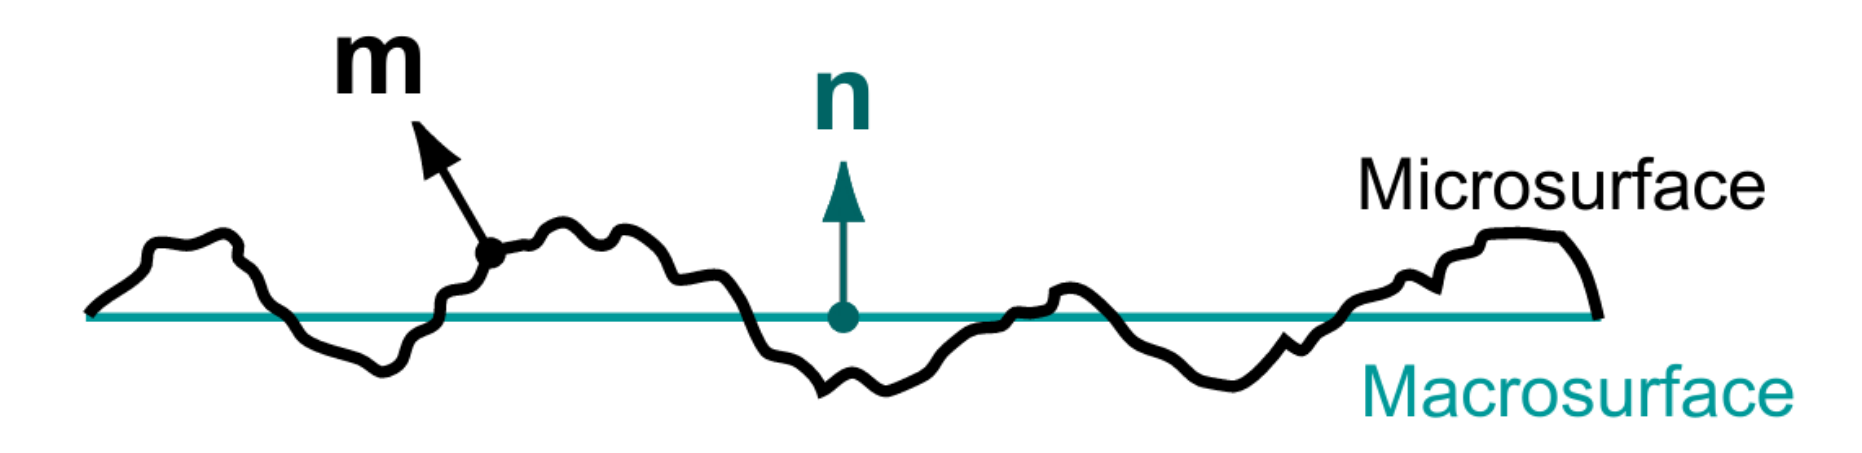
\includegraphics[width=0.5\textwidth]{Images/macro vs micro.png}
\caption{\label{micro-vs-macro}Micro vs macro surface \href{https://www.cs.cornell.edu/\~srm/publications/EGSR07-btdf.pdf}{(Source)}}
\end{figure}

Blenders implementation breaks down this down into two separate functions
by assuming that the microsurface can be adequately described using a microfacet
distribution function and a shadowing-masking function.

Blender provides these options for the distribution and shadowing functions, and
the subsurface methods.
\begin{itemize}
\item Distribution\footnote{Note that the \texttt{Distrubution} option Blender gives is different from the
\texttt{Microfacet Distrubution Function}, and includes both the \texttt{MDF} and the
Shadow-masking function.}
\begin{itemize}
\item GGX \\
\texttt{GGX} is a \texttt{BRDF} (bidirectional reflection distribution function) which
aims to be a faster than its alternative \texttt{Multiple-scattering GGX} however
at the cost  of physical accuracy.
The \texttt{MDF} describes the distribution of microsurface normals \textbf{m} (Figure
\ref{micro-vs-macro}) while the shadow masking function describes what fraction of
the microsurface normals \textbf{m} are visible. \cite{ggx-paper}

In \texttt{GGX} the shadow masking function does not account for reflections or
scattering. This can create excessive darkening and a loss in energy
conservation in some areas \cite{principled-bsdf-docs}.

\item Multiple-scattering GGX \\
Almost all popular parametric \texttt{BSDF}'s consider only single reflection
to account for self-shadowing and omit outgoing light that scatters
multiple times between microfacets. Omitting outgoing light  breaks
conservation of energy and leads to dark patches within rough surfaces
\cite{ms-ggx-paper}.
\begin{figure}[htbp]
\centering
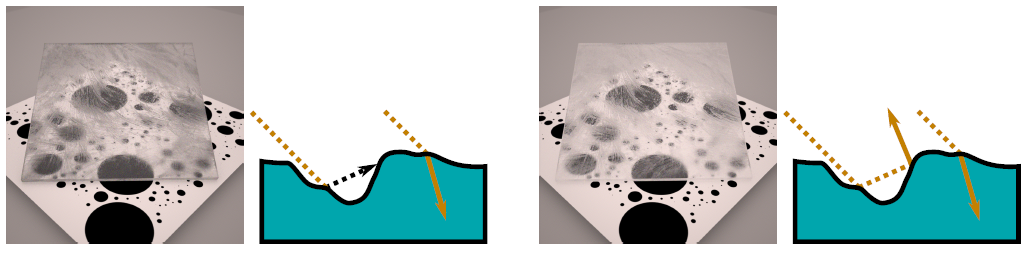
\includegraphics[width=.9\linewidth]{Images/multiplescatteringsmith_teaser.png}
\caption{Single scattering (left), multiple scatters (right), \href{https://eheitzresearch.files.wordpress.com/2015/10/multiplescatteringsmith\_teaser.png}{(Source)}}
\end{figure}

Blenders \texttt{Multiple-scattering GGX} \texttt{BRDF} allows for multiple light bounces
within microfacets to achieve 100\% energy conservation and provide a more
physically accurate render \cite{principled-bsdf-docs,ms-ggx-paper} . It
accomplishes this by conducting a random walk on the microsurface until the
ray escapes. Unlike \texttt{GGX} there is no known analytical expression for this
model (Blender's specific implementation), it must instead be solved
stochastically \cite{blender-issue-tracker}.
This comes at a performance cost, the original papers cites a 19\% penalty
using a Monte Carlo physically based renderer, Blenders development forums
estimates the performance penalty to be approximately 3\% at the time of
implementation \cite{blender-issue-tracker}.
\end{itemize}

\item Subsurface Scattering Method\\
Subsurface scattering is when light penetrates into an object that is normally
opaque and interacts and exits the material at a different point. Described
by a \texttt{BSSRDF} (bidirectional subsurface scattering reflectance distribution
function)
\begin{itemize}
\item Christensen-Burley \\
The \texttt{Christensen-Burley} method is an approximation of a physically based
volumetric scattering system with faster evaluation and efficiency \cite{Christensen-Burley}.
\item Random walk \\
Opposed to the approximations use the in the \texttt{Christensen-Burley} model,
the \texttt{Random walk} modelling uses true volumetric scattering inside the mesh.
Due to this the model does not perform well when the mesh is not closed.
This accuracy comes at a cost of rendering time (actually performance hit is largely
dependent on the model itself), and increased noise.

Accuracy within the subsurface scattering was not an area of importance
within this report thus the \texttt{Christensen-Burley} model was chosen due to
its better performance.
\end{itemize}
\end{itemize}

All renders within this report have \texttt{Multiple-scattering GGX} enabled as the
benefit outweighed the cost.

The \texttt{Principled BSDF} shader is a combination of multiple layers into a single
node. This is done for ease of use.

This shader encapsulates bidirectional reflectance and transmittance
distribution functions. Individually these functions determine how light behaves
on the surface and inside a material.


\subsubsection{Pieces}
\label{sec:orga976a1f}
Pieces were modelled after the reference image below Figure \ref{piece-reference}.
From this image the pieces where traced using the \texttt{Add Vertex} tool, from the
\href{https://docs.blender.org/manual/en/2.92/addons/add\_mesh/mesh\_extra\_objects.html}{Add Mess Extra Objects} add-on. To transform this line of vertices to a solid
object  a \texttt{Screw} modifier was applied.
\begin{figure}[htbp]
\centering

\includegraphics[width=0.5\textwidth]{ref/bee5aa3d08a30da4ca1005cbd0fe10b54a03bb49.jpg}
\caption{\label{piece-reference}Reference image, Licensed under \href{https://pixabay.com/service/license/}{Pixabay License}}
\end{figure}

\begin{center}
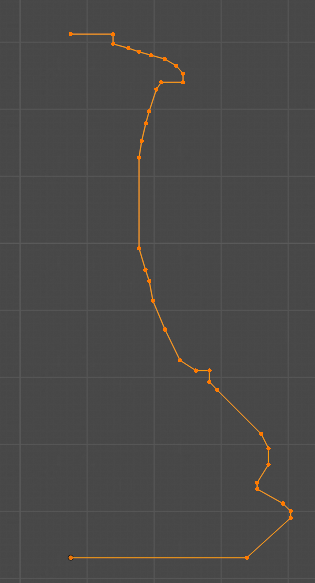
\includegraphics[height=150pt]{Images/modelling piece inprogress.png}
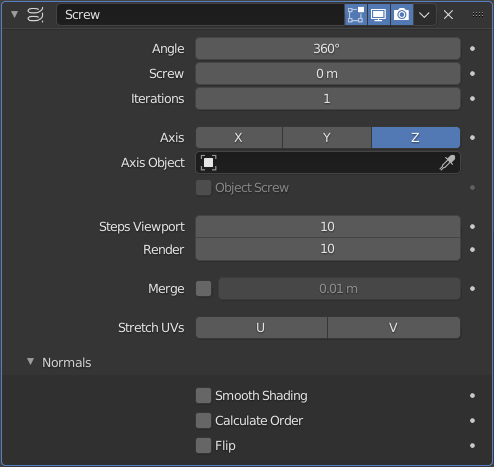
\includegraphics[height=150pt]{Images/screw settings.png}
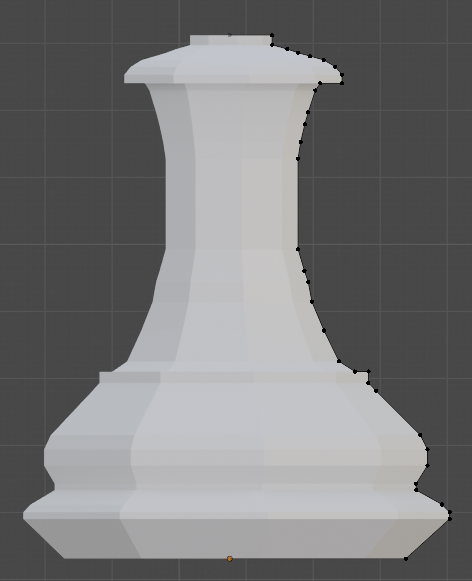
\includegraphics[height=150pt]{Images/pawn model.png}
\end{center}
The notable changes from the default settings is the lowering of the steps from
\(16 \to 10\) and disabling \texttt{Smooth Shading}. This was a stylistic choice as the
low polygon look would better demonstration reflections and the planned indirect
lighting (See \hyperref[sec:orgee3f3d9]{Lighting - Disco Ball}).\\

To model the knight, 3 separate reference images where used. The base was
constructed in a similar manner to the other pieces. The head was modelled
manually.

\begin{figure}[htbp]
\begin{center}
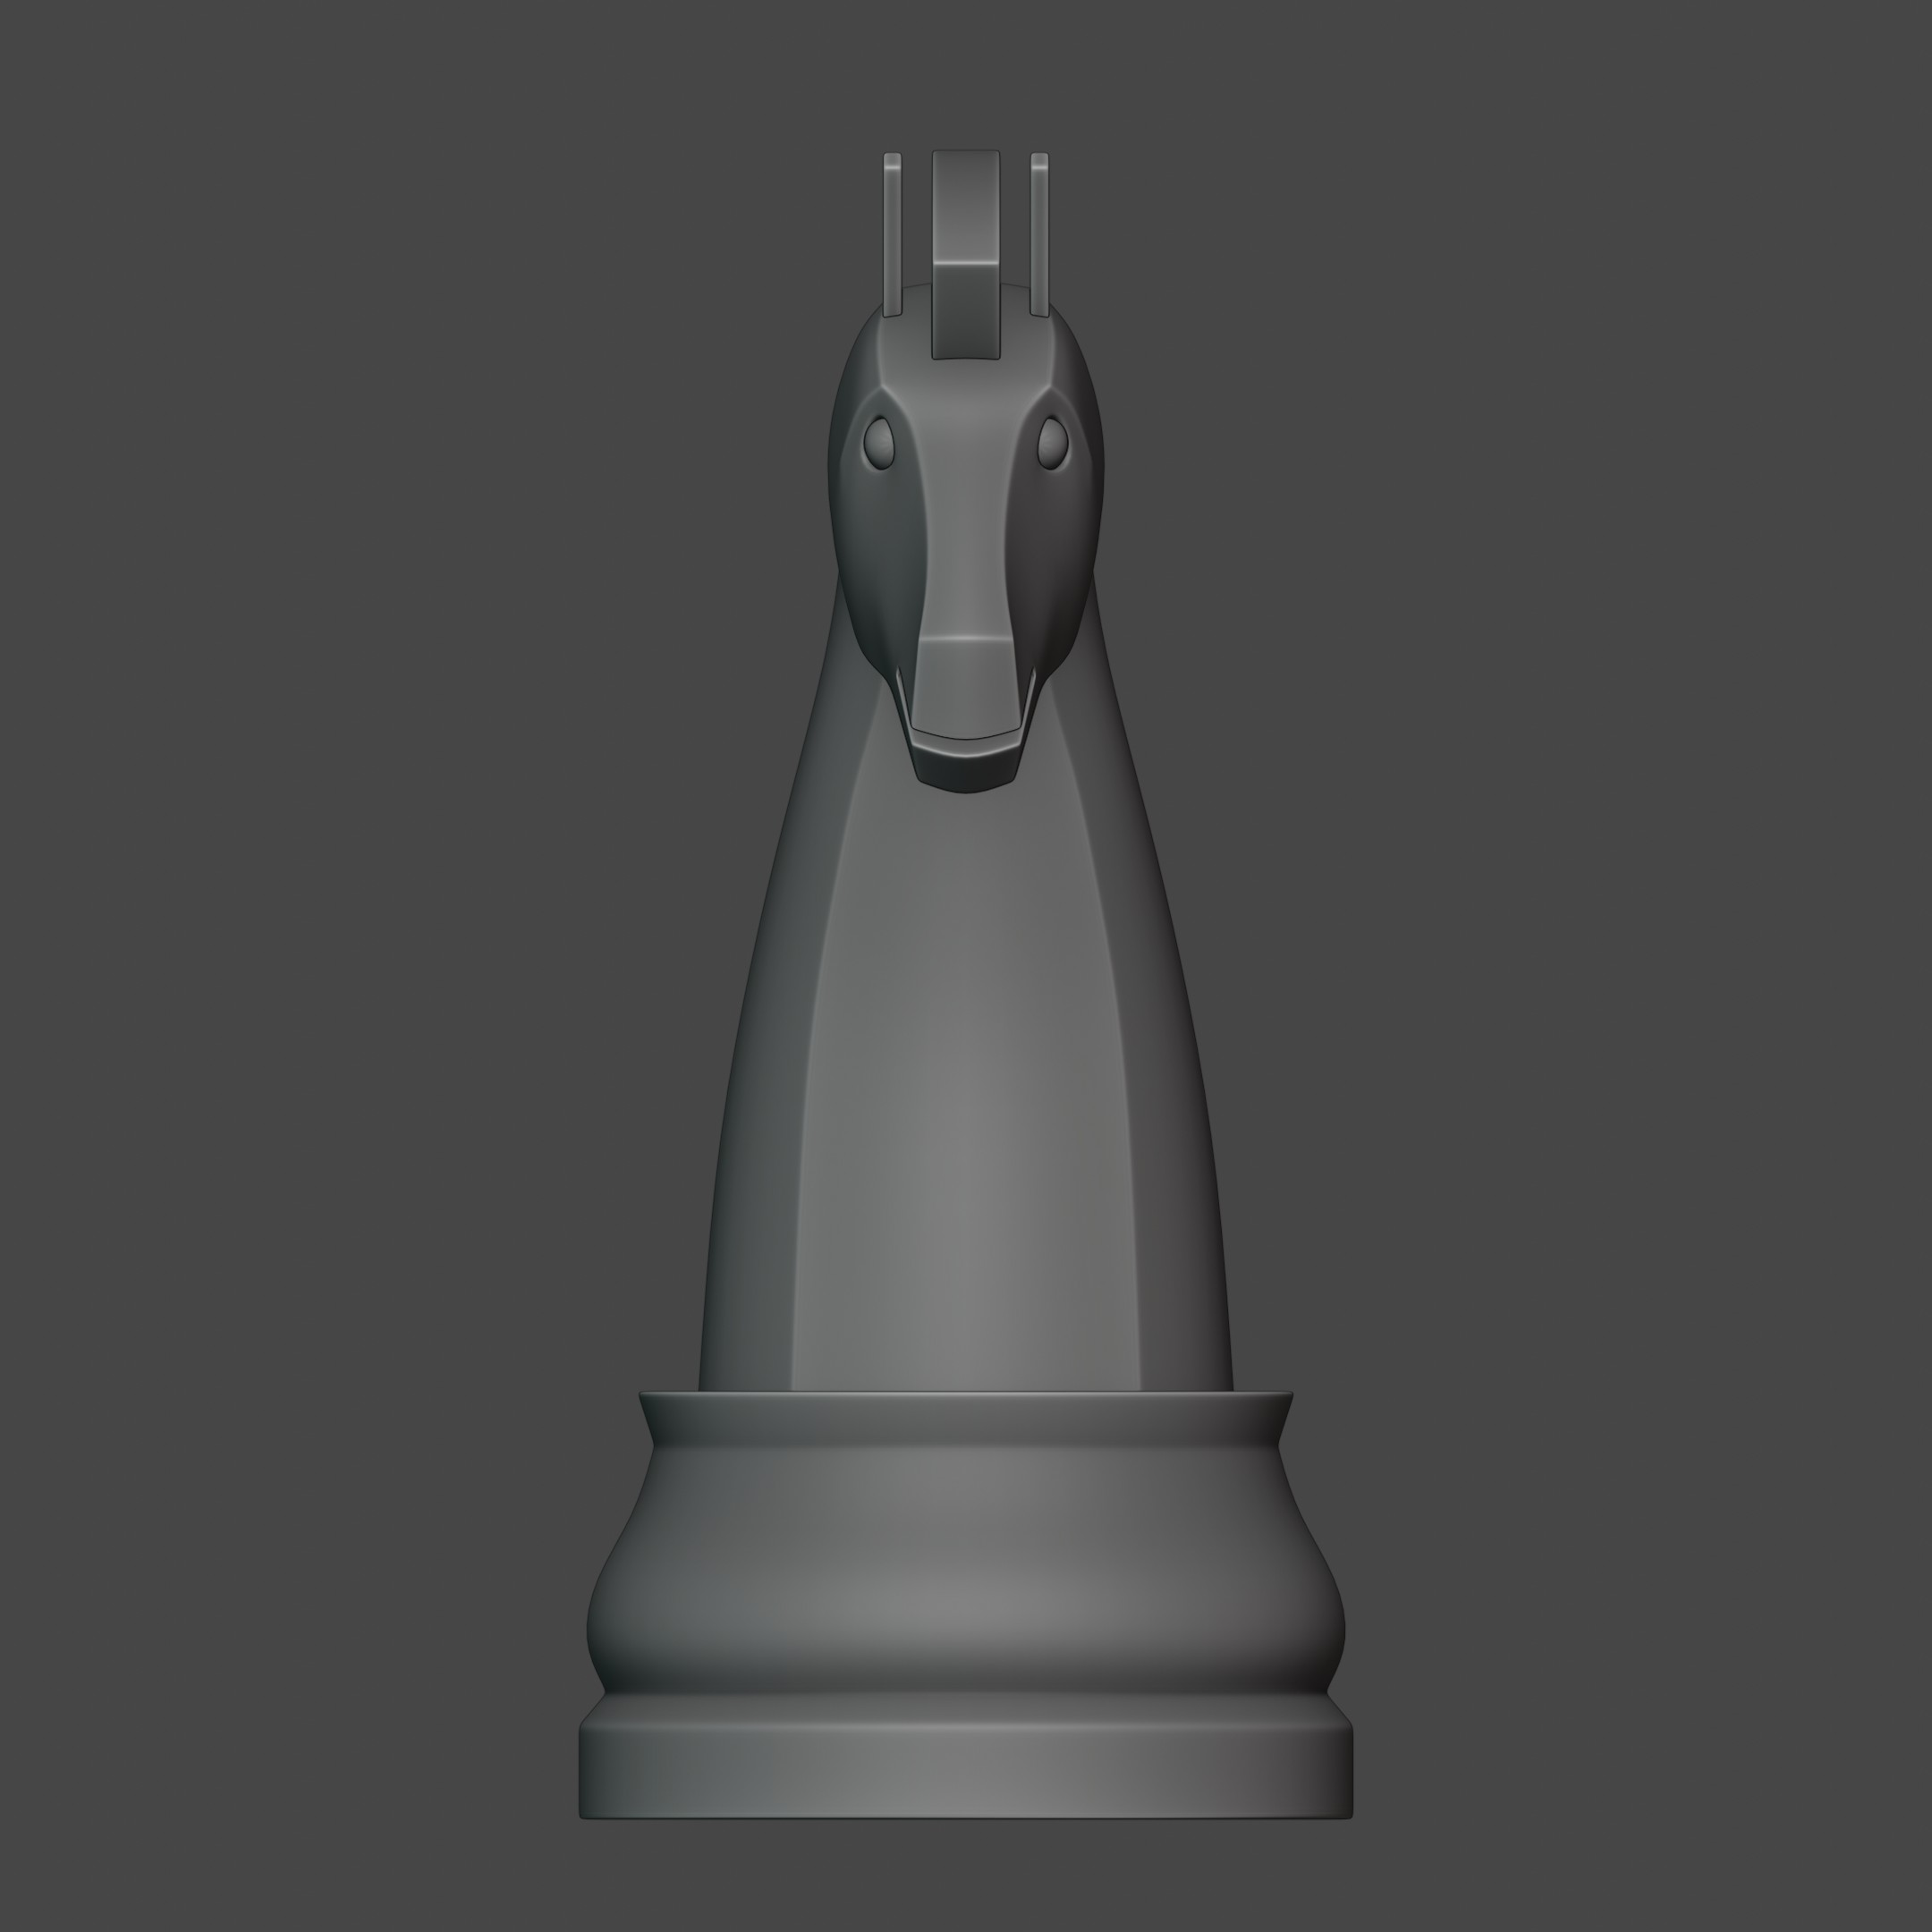
\includegraphics[width=0.3\textwidth]{ref/knight front.jpg}

\includegraphics[width=0.3\textwidth]{ref/knight right.jpg}
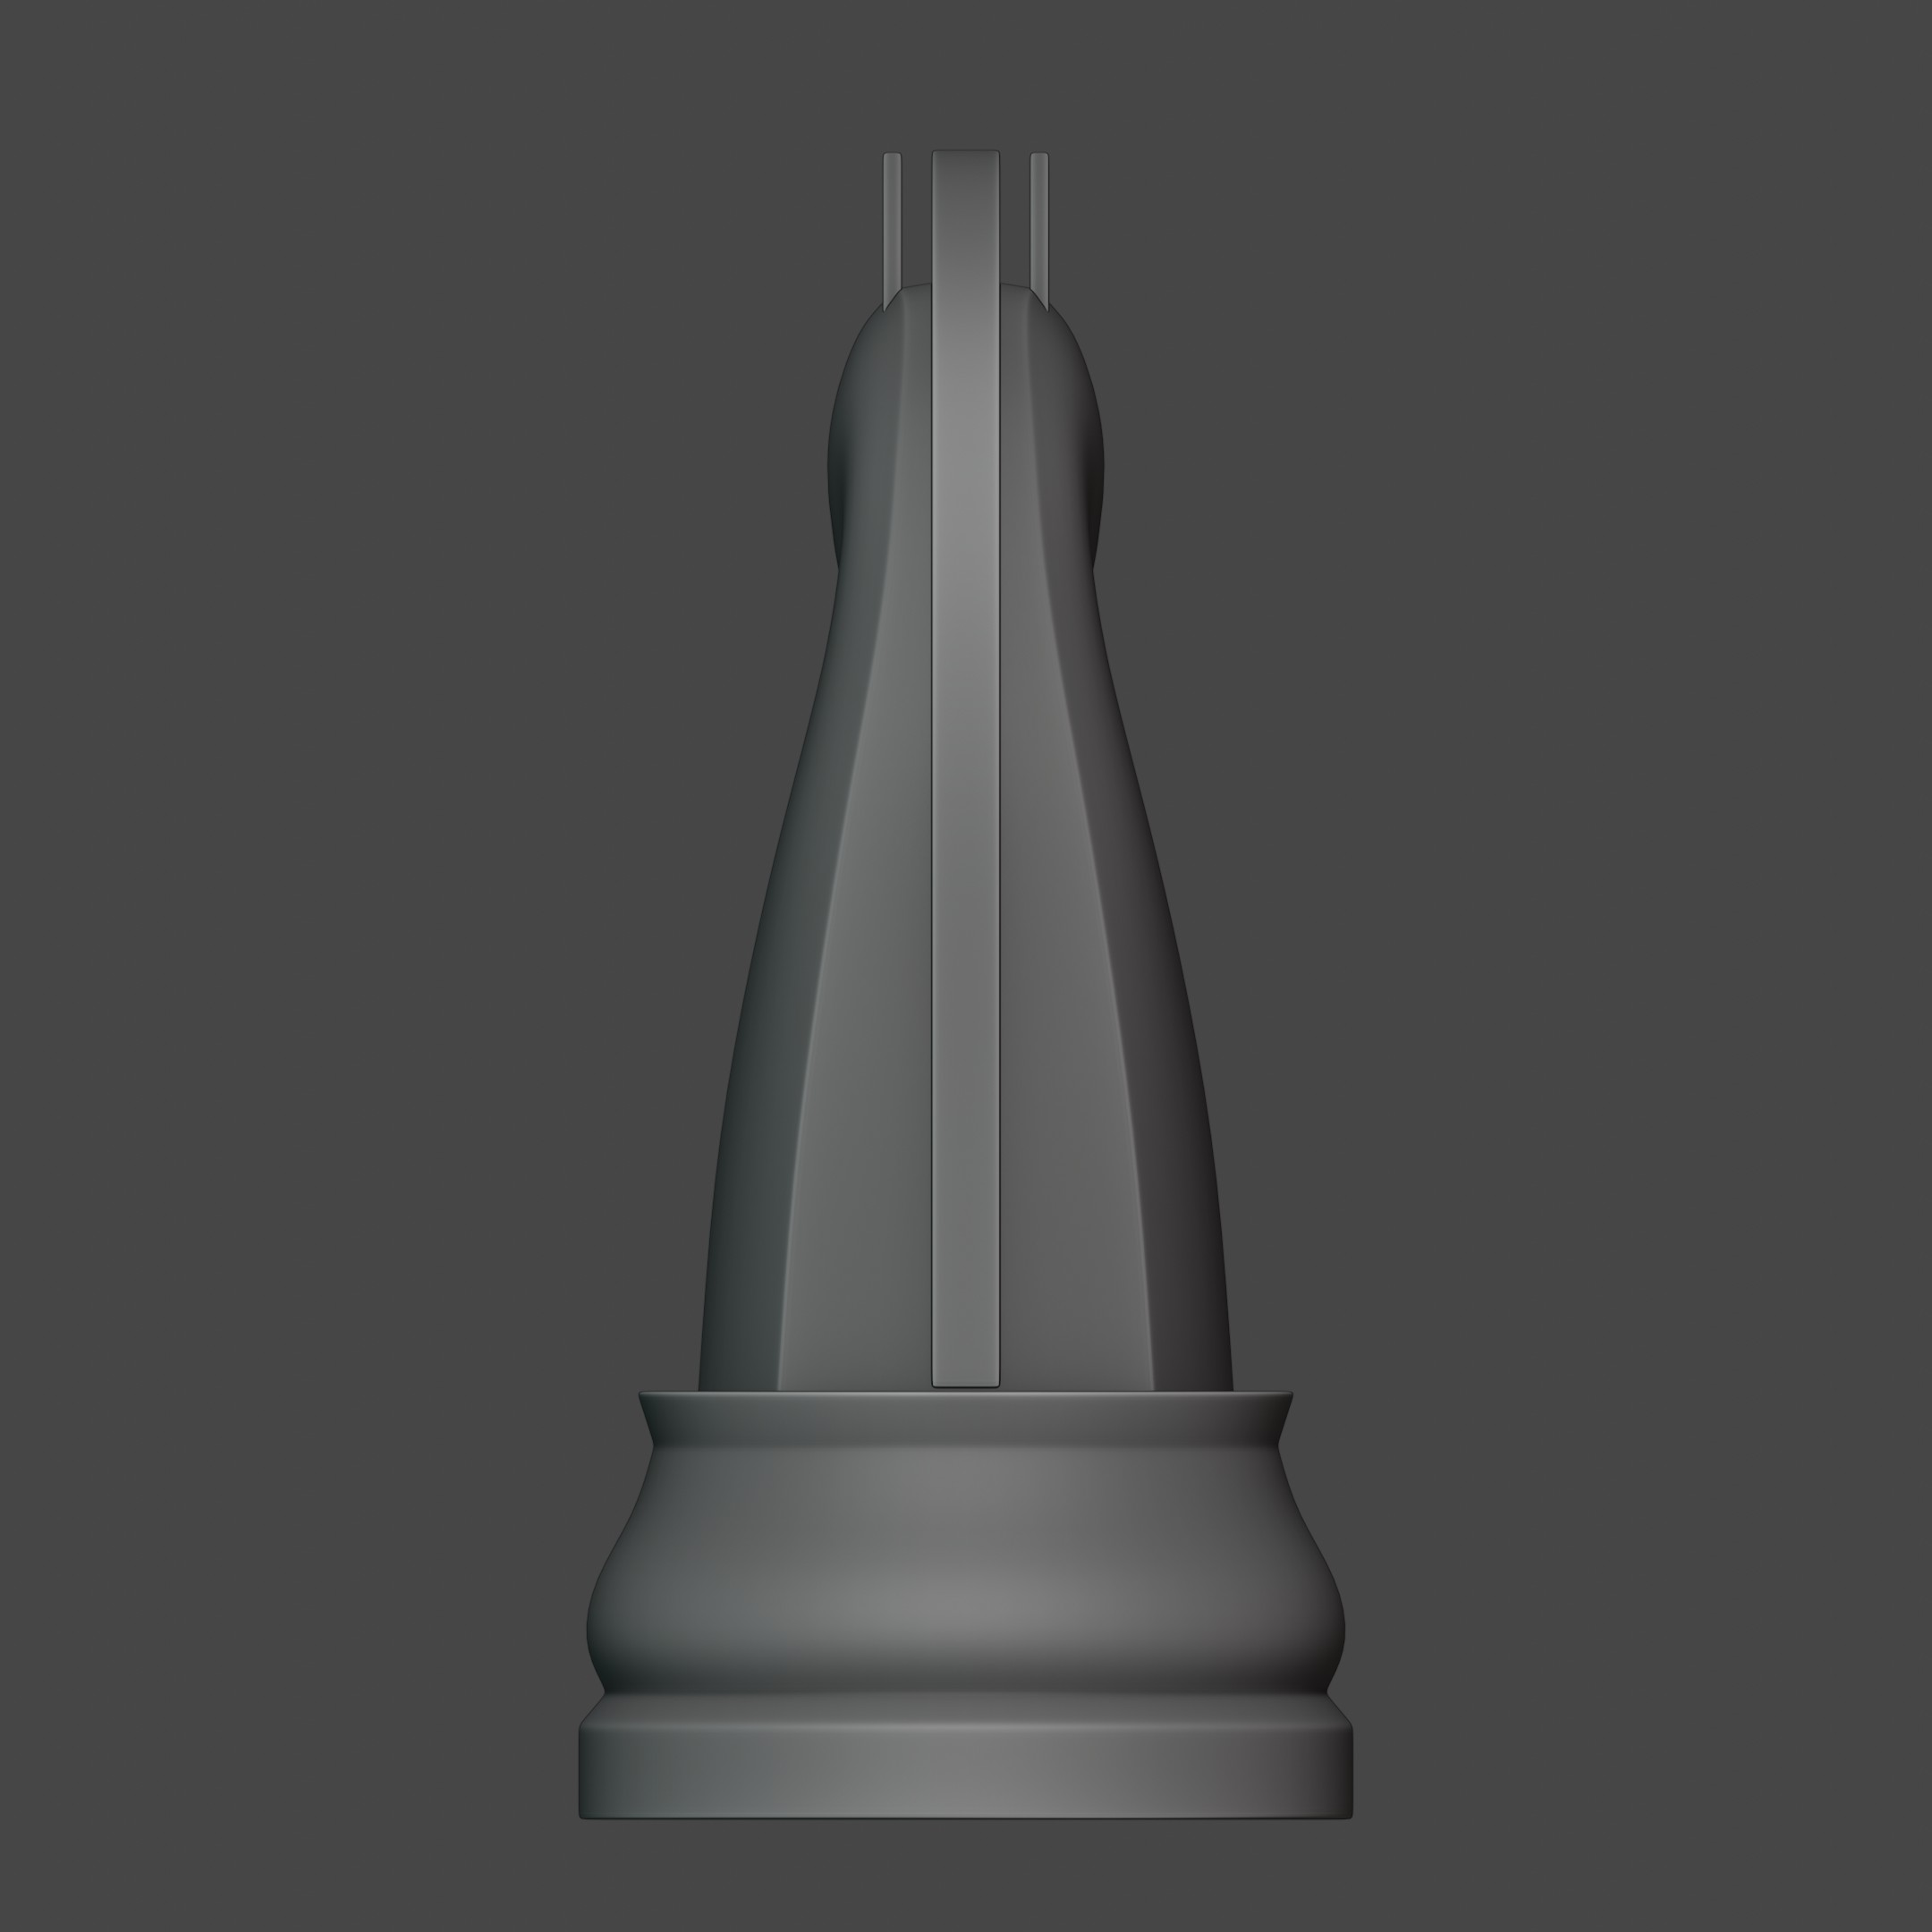
\includegraphics[width=0.3\textwidth]{ref/knight back.jpg}
\end{center}
\caption{Knight reference images, \href{https://imgur.com/a/Pg9WYII}{(Source)}}
\end{figure}

Additionally ico-spheres where added to some pieces for additional detail.\\

The final piece models appear as below.
\begin{figure}[htbp]
\centering
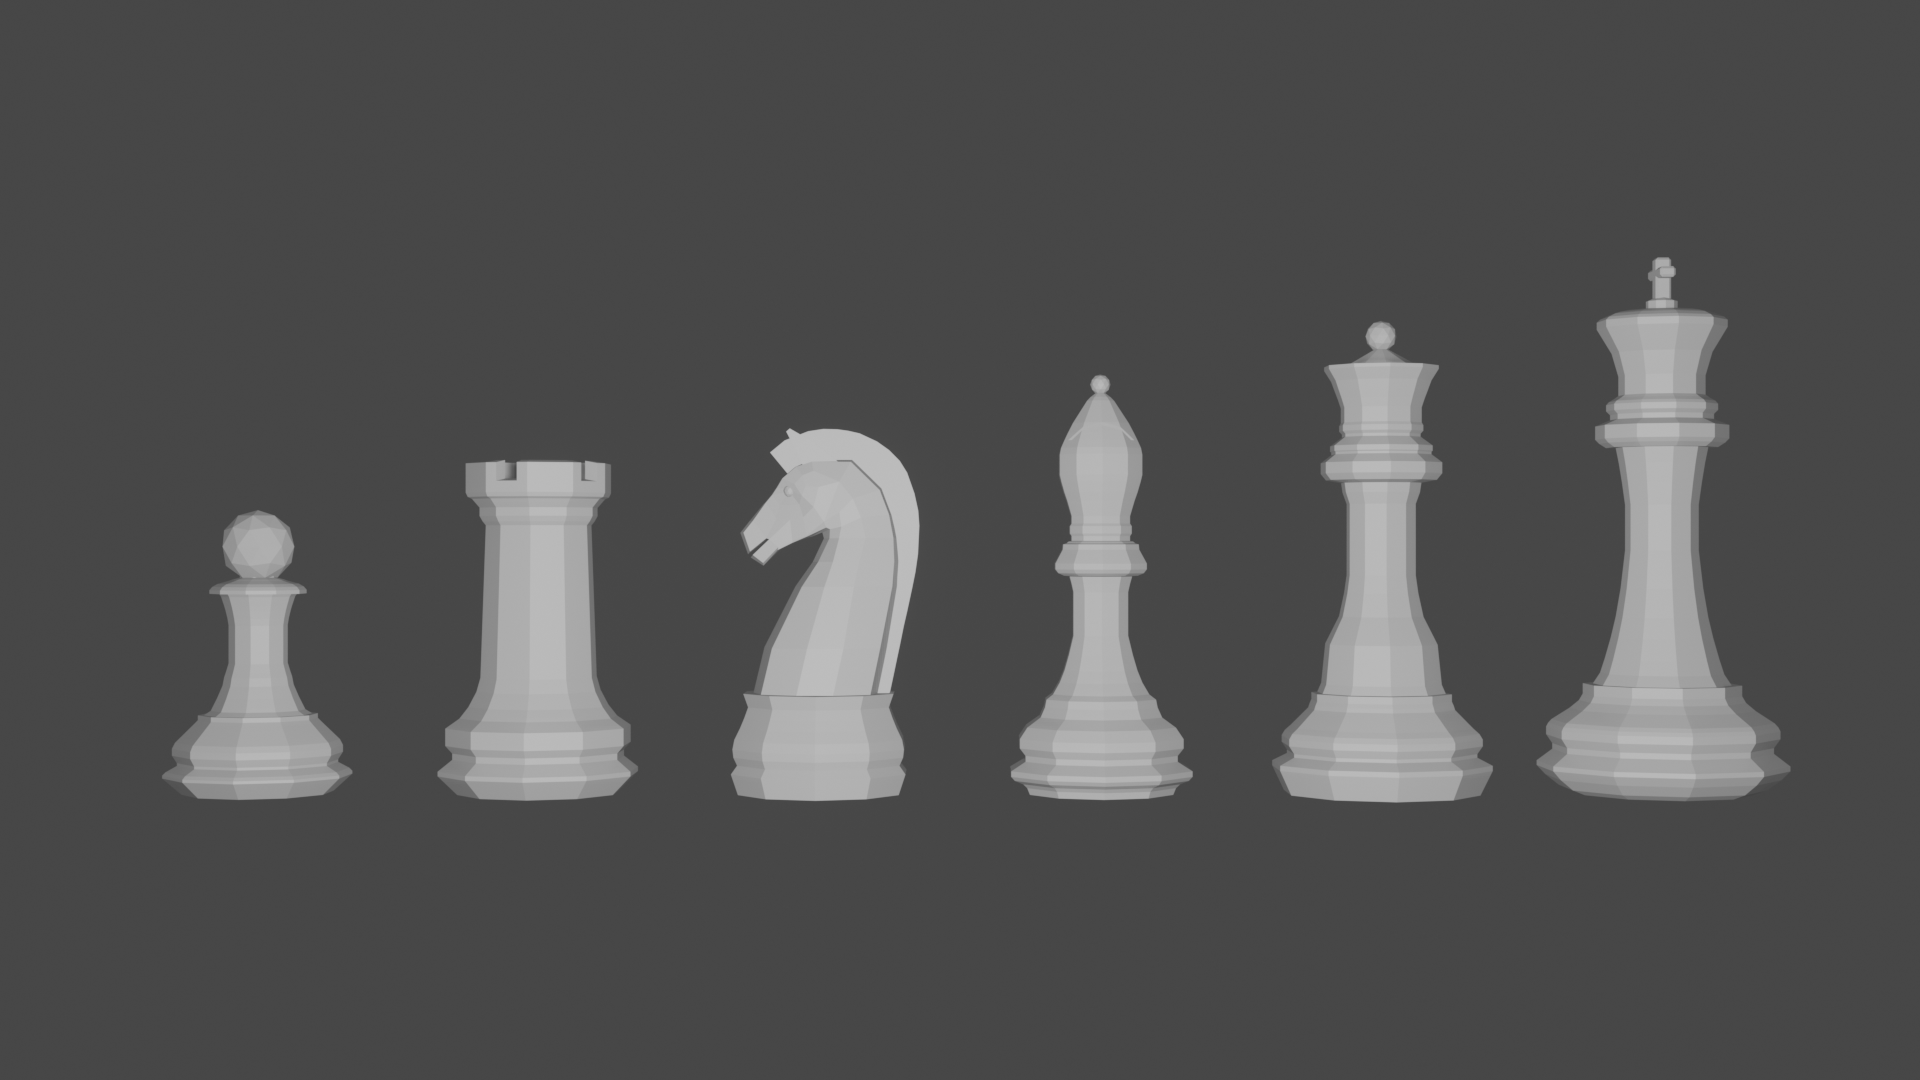
\includegraphics[width=0.5\textwidth]{Images/Pieces.png}
\caption{Final models}
\end{figure}
\newpage


\subsubsection{Board}
\label{sec:orgd304f7f}
\paragraph{Chess board}
\label{sec:org0ee51fb}
The chess board model is a simple rectangular based prism with dimensions \texttt{8m x
8m x 0.4m}. The checker board texture comes from the \texttt{Checker Texture}, with
\texttt{scale=8.0} and black and white colours. This texture output is fed into
the base colour input of a \texttt{Principled BSDF} shader node.\\

\begin{figure}[htbp]
\centering
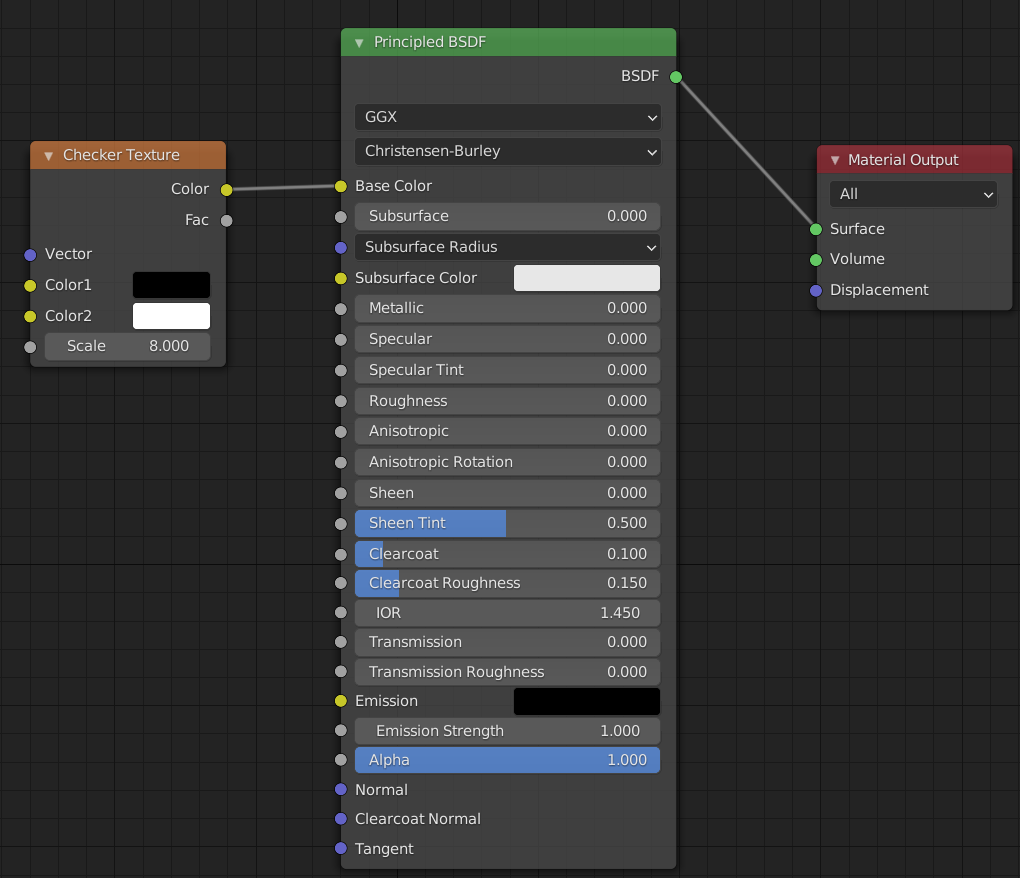
\includegraphics[width=350pt]{Images/checker texture.png}
\caption{\label{checker-texture}Complete checker board texture.}
\end{figure}

Within world space the board was positioned in the positive positive quadrant
such that the very bottom left handle corner of the board was at \texttt{0,0}
with each squares dimensions as \texttt{1m x 1mx}. This positioning becomes important
in \hyperref[sec:org3045217]{Python implementation - Array index to world space}.
\newpage
\paragraph{Marble exterior}
\label{sec:orgb9c464d}
\begin{wrapfigure}[12]{r}{0.3\textwidth}
\centering
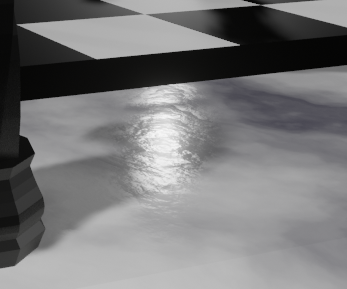
\includegraphics[width=0.2\textwidth]{Images/normal.png}
\caption{\label{marble-normal-texture}Marble normal texture}
\end{wrapfigure}

The marble exterior was added to showcase reflections, shadows, bloom, and specular
highlights through the use of procedural texture and normal mapping.\\

To accomplish this texture layered Perlin noise was used. The first set of
switch derives its coordinators from the \texttt{Texture Coordinate} node which is set
to use the mesh \footnote{A very interesting effect can be achieve by using the \texttt{Camera} as the
source of the coordinates. The marble texture flows like sea foam as the camera spins.}. The \texttt{Mapping} node is extraneous in this example, simply
used to move the Perlin noise map around. The second layer of Perlin noise uses
the already nosy surface to create the dark patches marble typically features.
The colour ramp is used to brighten and shade the darker patches of noise. This
colour is then used as the base colour for the \texttt{BSDF} shader. To give this
texture some depth the colour output of the ramp is used to create a normal map.
Colour data (yellow node), when used as a vector input can yield unexpected results.
To remedy this the colour data is first passed through a \texttt{Bump} node as the height
data and then fed into the \texttt{BSDF} shader.
\begin{figure}[htbp]
\centering
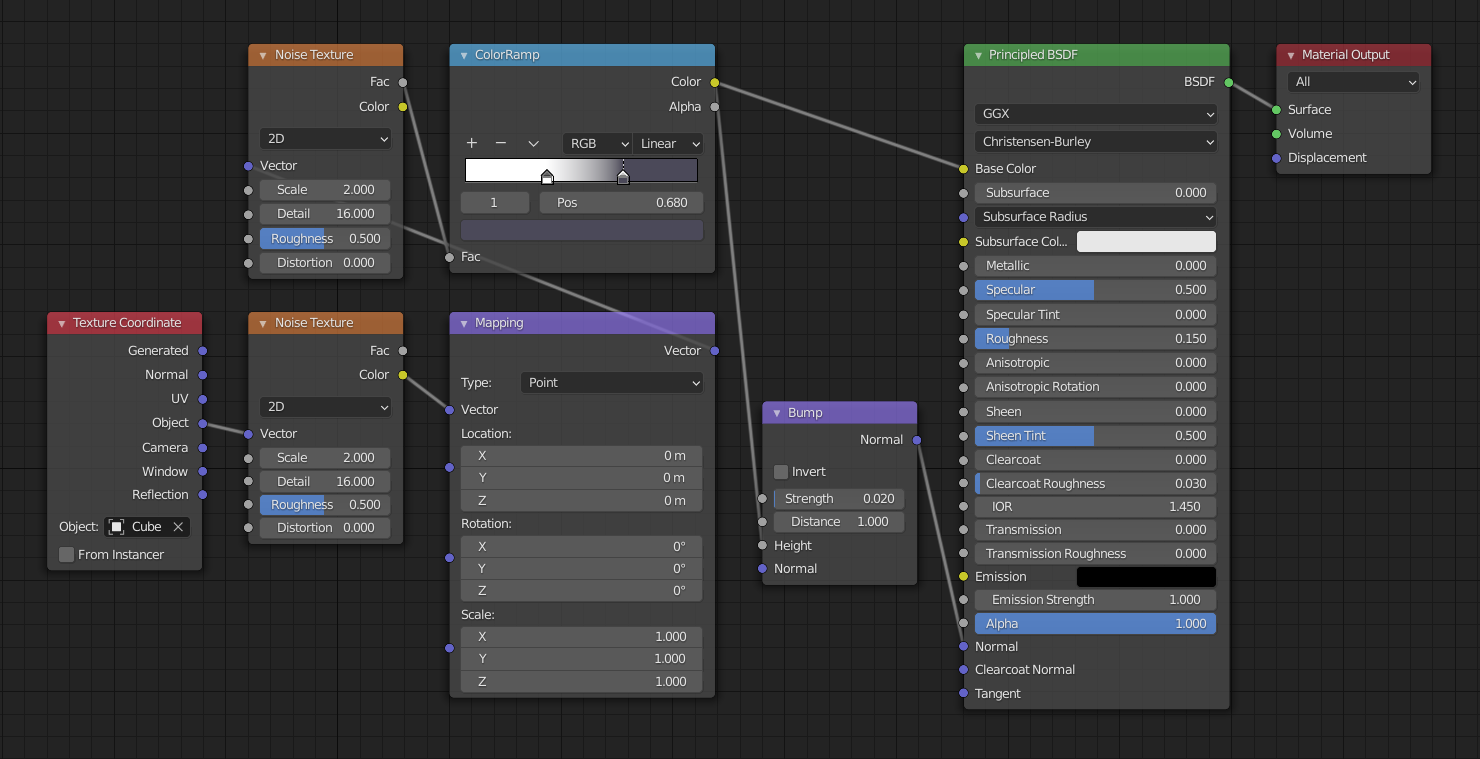
\includegraphics[width=\textwidth]{Images/marbletextire.png}
\caption{\label{marble-texture}Complete marble texture}
\end{figure}

\begin{figure}[htbp]
\centering
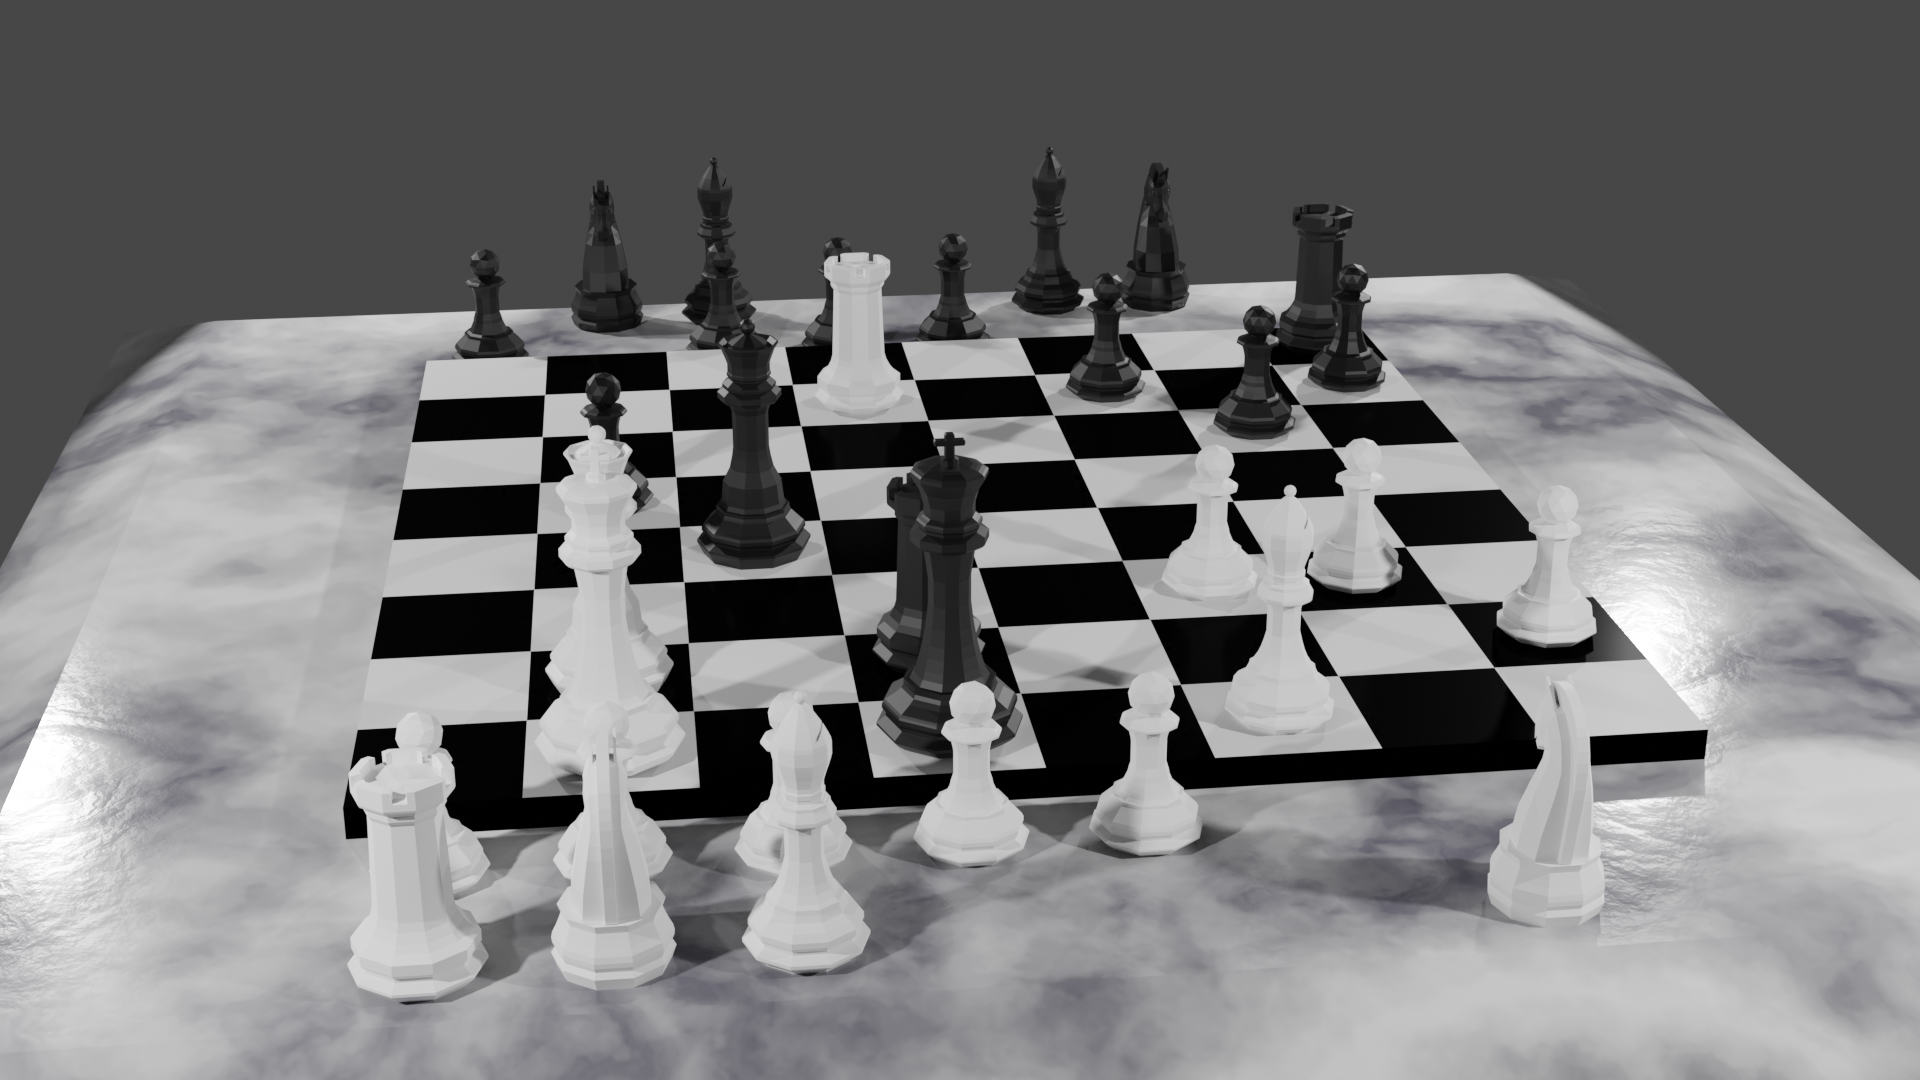
\includegraphics[width=\textwidth]{Images/Marble cycles.png}
\caption{Cycles marble render}
\end{figure}

\begin{figure}[htbp]
\centering
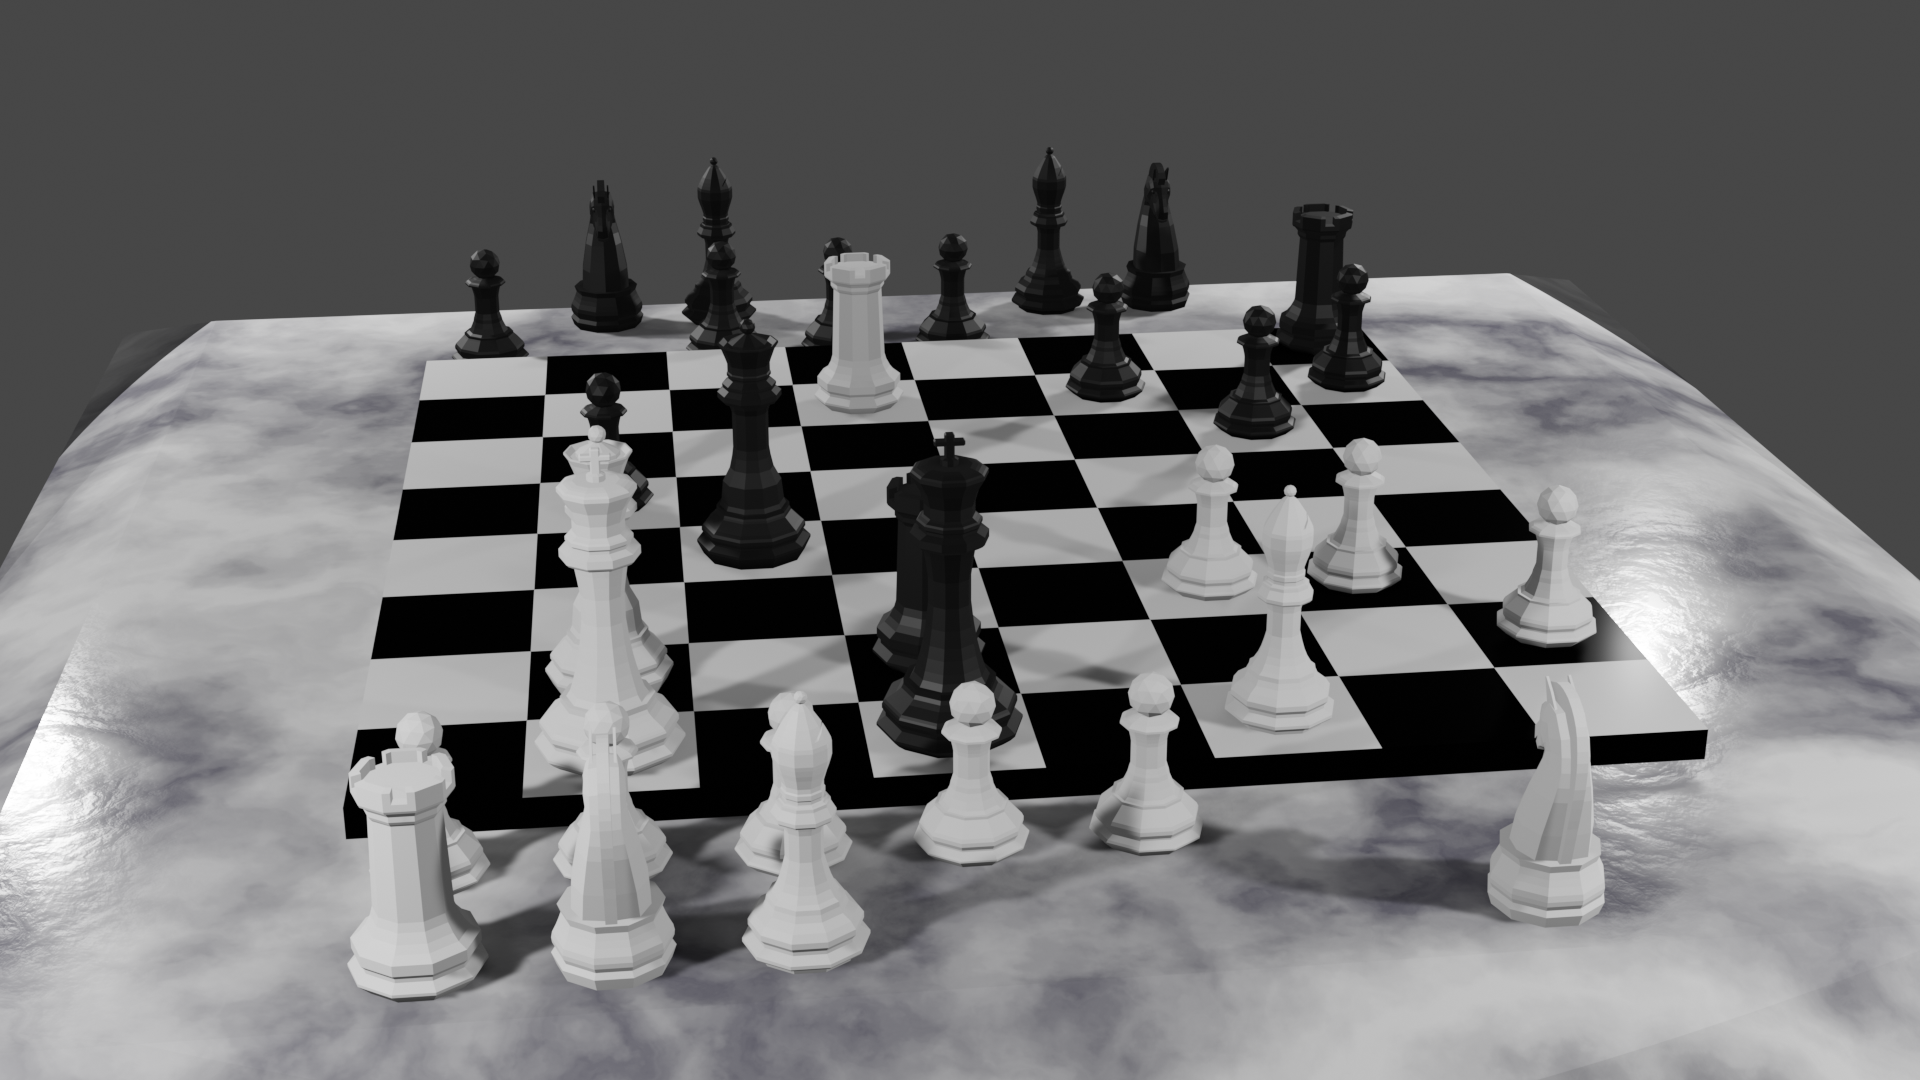
\includegraphics[width=\textwidth]{Images/Marble eevee.png}
\caption{Eevee marble render}
\end{figure}
\newpage
\subsection{Particle effects}
\label{sec:orgb851a90}
\subsubsection{Explosions}
\label{sec:org87d3464}
Initially an explosion was planned on each piece capture as a way to add some
flare. However this was quickly scrapped as the additional baking and rendering time
were deemed too costly. A demo render featuring a smoke cloud was created and can
be viewed here \href{https://github.com/Jake-Moss/blender-chess/blob/master/Videos/smoke.mp4}{master/Videos/smoke.mp4}.
\subsubsection{Confetti}
\label{sec:org697762f}
As an alternative to explosions, a confetti shower on the winning king (only
checkmates received confetti) was added instead.\\

The confetti is still an explosion but with the outgoing particles set to a
collection of ``confetti's''. The source of the explosion is a upwards facing
dome, this gives the confetti a even spread. The particles are set to have
randomised, size, rotation, angular velocity, and normal velocity. To achieve the
slow fall effect the effective gravity of the particle simulation was lowered to
38\% its normal strength. Each confetti has a texture with \texttt{Roughness 1.0} and
varying base colours.

\begin{figure}[htbp]
\begin{center}
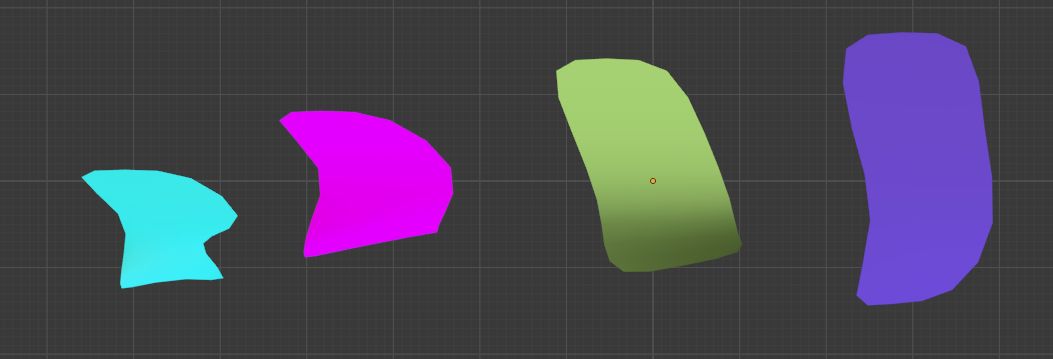
\includegraphics[width=0.5\textwidth]{Images/confetties.png}
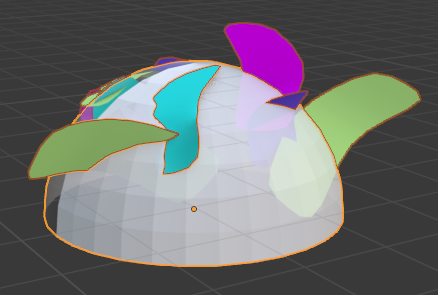
\includegraphics[width=0.3\textwidth]{Images/confetti dome.png}
\end{center}
\caption{Confetties (left), confetti source (right)}
\end{figure}

A sample render can be seen below.
\begin{figure}[htbp]
\centering
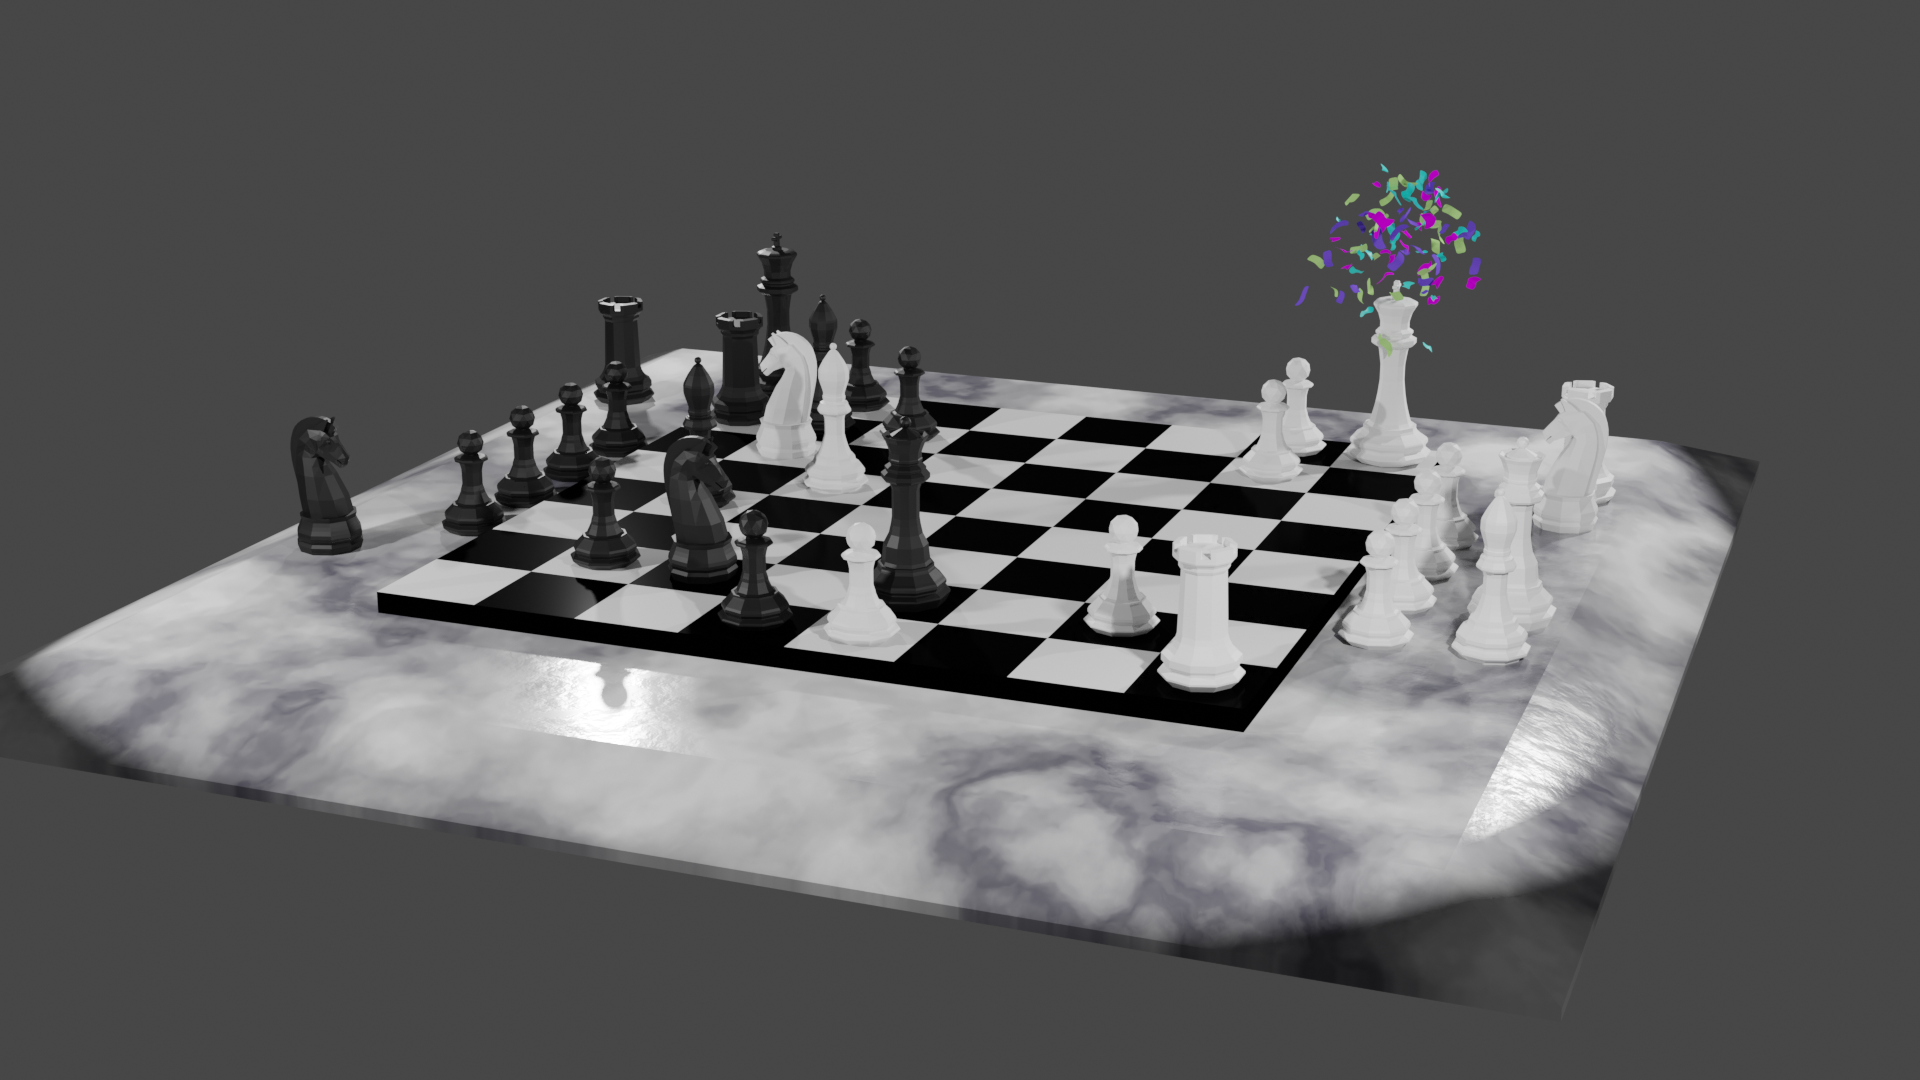
\includegraphics[width=\textwidth]{Images/Confetti! cycles.png}
\caption{Confetti render using Cycles}
\end{figure}
\newpage
\subsection{Lighting}
\label{sec:orgadc1a7c}
The power of Blender lights is measured in \texttt{Watts}, however this is not the same
wattage consumer lights bulbs are rated in. Blenders light power is rated
in radiant flux, which is the measure of radiant energy emitted per unit time
opposed to consumer light bulb which are rated in lumens, or luminous flux
\cite{radiant-flux,luminous-flux}. Luminous flux differs from radiant flux in that
luminous flux is adjusted to the varying sensitivity of the human eye.
\cite{luminous-flux}

\begin{table}[htbp]
\caption{Blender light power conversion \href{https://docs.blender.org/manual/en/latest/render/lights/light\_object.html\#power-of-lights}{(Source)}}
\centering
\begin{tabular}{lll}
\hline
\textbf{Real world light} & \textbf{Power} & \textbf{Suggested Light Type}\\
\hline
Candle & 0.05 W & Point\\
\hline
800 lm LED bulb & 2.1 W & Point\\
\hline
1000 lm light bulb & 2.9 W & Point\\
\hline
1500 lm PAR38 floodlight & 4 W & Area, Disk\\
\hline
2500 lm fluorescent tube & 4.5 W & Area, Rectangle\\
\hline
5000 lm car headlight & 22 W & Spot, size 125 degrees\\
\hline
\end{tabular}
\end{table}

\subsubsection{Direct}
\label{sec:org52578a3}
To directly light the scene four spot lights were placed at the corners of the
board. Spot lights were chosen instead of typical point lights or sun
lights to give consistent directional lighting during the camera spins. The four
lights are set to track the centre of the chess board.
\begin{figure}[htbp]
\centering
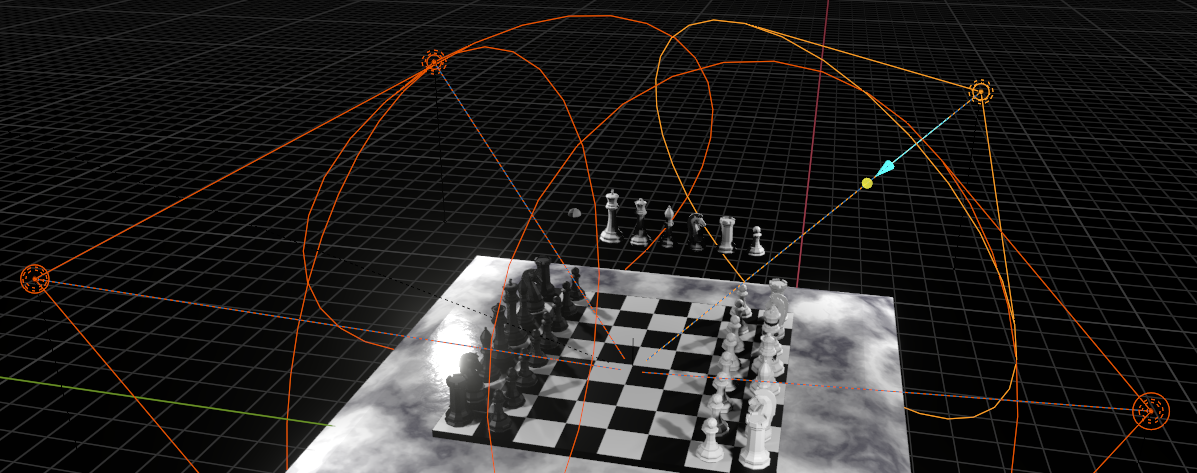
\includegraphics[width=\textwidth]{Images/lighting.png}
\caption{Spot light positions}
\end{figure}
To account for the unrealistic scale the power of the lights was set to higher
than normal. However, this was still not enough. To avoid cranking the lights
to approximately \texttt{1MW} the exposure within the film settings was adjusted to
compensate as per the Blender documentation \cite{light-power-docs}.

The blend for this light was set to 0 as the cone fully encompasses the board.
\subsubsection{Indirect}
\label{sec:org99f981f}
There is minimal indirect lighting within the final scene (all models
reflect some amount of light due to their texturing, however this is not a
significant amount). Considering this a second scene was created which featured
considerable indirect lighting. To accomplish this a disco ball was implemented.
\paragraph{Disco ball}
\label{sec:orgee3f3d9}
Whats better than chess? That's right, disco chess! There is no better way to
demonstrate indirect lighting that a giant ball of mirrors in the middle of the board.

The disco ball model is a simple iso-sphere with a mirror like texture. Its
rotation is achieved through simple key-frames.

To create a mirror in Blender the \texttt{Roughness} parameter on the \texttt{Principled BSDF}
shader node is set to 0. This alone didn't make a very convincing disco ball, in
addition to the \texttt{Roughness}, the following values were tweaked,
\begin{itemize}
\item \texttt{Metalic 1.0}\\
This change made the ball most disco like as it gives a fully specular
reflection tinted with the base colour without diffuse reflection or
transmission.
\item \texttt{Specular 1.0}\\
While the \texttt{Matallic} value is responsible for the majority of the specular
reflection, this change gave the ball a halo like glow.
\item \texttt{Base colour}\\
With the two previous changes the disco ball appeared too uniform and reflective, some
faces appeared completely blown out with no variance between them. To remedy
this a \texttt{Voronoi} noise texture's colour output was piped into a colour ramp
(this is done to avoid the \textbf{very} pink look  the \texttt{Voronoi} noise produces).
\end{itemize}

\begin{figure}[htbp]
\centering
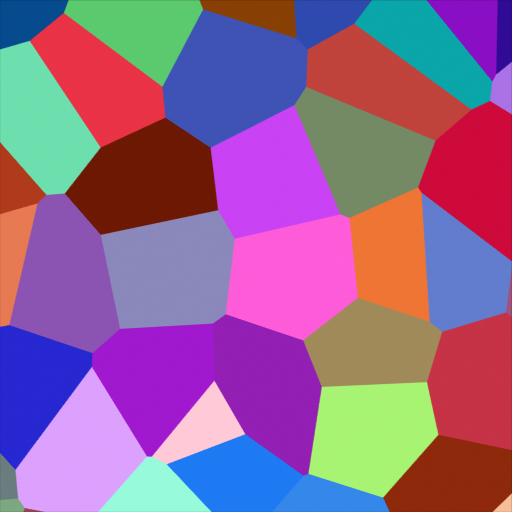
\includegraphics[width=0.3\textwidth]{Images/render_shader-nodes_textures_voronoi_smoothness-color-zero.png}
\caption{\texttt{Voronoi} texture colour output}
\end{figure}
A \texttt{Voronoi} noise texture is as procedural \href{https://en.wikipedia.org/wiki/Worley\_noise}{Worley noise} function evaluated at the texture
coordinate. The patterns are generated by randomly distributing points. From
these points a region is extended, the bounds of this region is determined by
some distance metric. The standard Euclidean distance is used here.

\begin{figure}[htbp]
\begin{center}
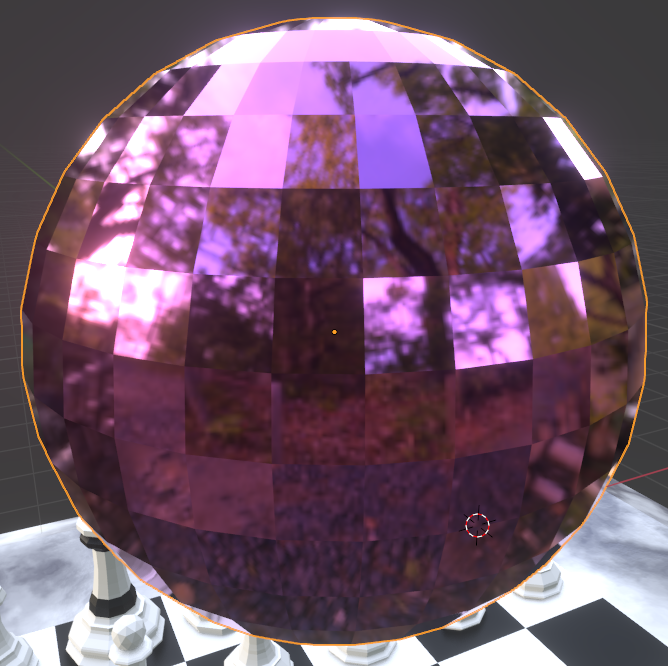
\includegraphics[width=0.3\textwidth]{Images/Purple.png}
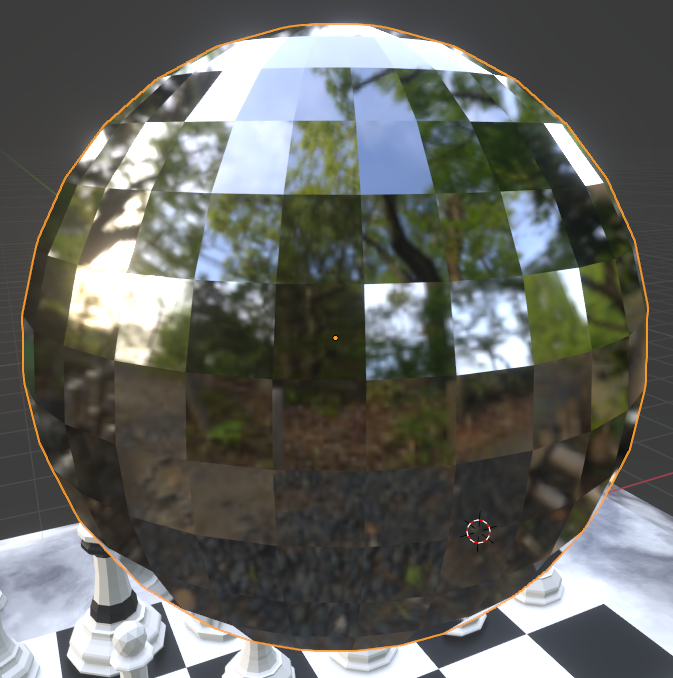
\includegraphics[width=0.3\textwidth]{Images/discoclose.png}
\end{center}
\caption{No colour ramp (left), complete texture (right)}
\end{figure}

\begin{figure}[htbp]
\centering
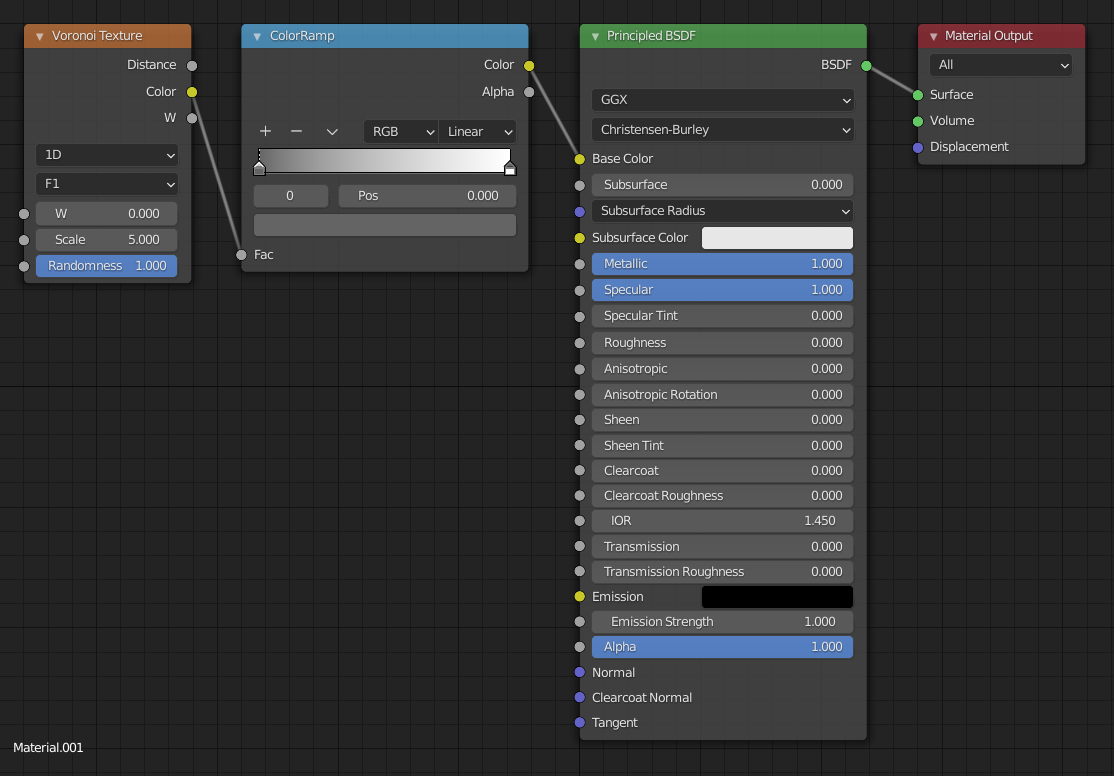
\includegraphics[width=0.7\textwidth]{Images/discoball_texture.png}
\caption{Complete disco ball texture}
\end{figure}
\newpage
With the disco ball texture and model complete a two red and blue lights were
trained on the disco ball. The results can be seen with the \hyperref[sec:orgc163b91]{Render engine section}.
\subsection{Render engine}
\label{sec:orgc163b91}
Blender offers two modern rendering engines, when working on a project it is
important to keep in mind what engine will be used for the finally render in ord
to account for the limitations of both. For this project \texttt{Eevee} was the chosen
engine due to the significantly lower render times than \texttt{Cycles}, however
renders using both engines were still made in order to compare them.\\

This project also made use of third engine, \texttt{Luxcore}. \href{https://luxcorerender.org/}{\texttt{Luxcore}} is a free and
open source rendering engine designed specifically to model physically accurate
light transportation.
\newpage
\subsubsection{Eevee}
\label{sec:org7013092}
Blenders \texttt{Eevee} is designed to be used within the view port for real time rendering previews
\texttt{Eevee} must cut corners to achieve this speed. Although these
approximations are physically based, the behaviour of light suffers. By default
mirrors do not function (without explicitly enabling) and caustics are not present at all.\\

\texttt{Eevee}'s pipeline, while \href{https://wiki.blender.org/wiki/Source/Render/EEVEE/GPUPipeline}{lacking signifcant documentation}, is that of a typical
rasterisation engine.
\begin{figure}[htbp]
\centering
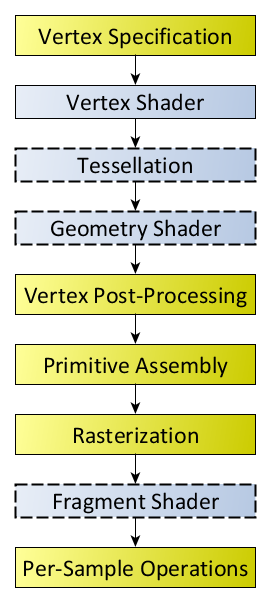
\includegraphics[width=0.3\textwidth]{Images/RenderingPipeline.png}
\caption{\label{rendering-pipline-eevee}Rendering pipeline \href{https://www.khronos.org/opengl/wiki/File:RenderingPipeline.png}{(Source)}}
\end{figure}

\begin{enumerate}
\item Vertices are retrieved from the buffer object \footnote{A buffer object is an array of unformatted memory allocated by the GPU.}. This includes vertex
colours, UV coordinates, and vertex locations of polygons.
\begin{enumerate}
\item The retrieved vertices are transformed to the post-projection space by the
vertex shader.
\item (Optional) Tesselation is where patches of vertex data are subdivided into
smaller interpolated points. This is useful to dynamically add or subtract
detail from a polygon mesh.
\item (Optional) The geometry shader is used to conduct layered rendering which is
useful when cube based shadow mapping or rendering a cube enrichment map
without having to render the entire scene multiple times.
\end{enumerate}
\item Vertex post-processing - output from the previous stages is collected
and prepared for the following stages.
\begin{enumerate}
\item In Transformation Feedback the output of the Vertex Processing stages is
recorded and placed into buffer objects, preserving the post-transformation
rendering state such that it can be resubmitted to various processes.
\item Primitive Assembly prepares the primitives for the rasterizer by dividing
them into a sequence of triangles and stored in an efficient method.
\item Geometry outside of the view is culled and vertices are transform from NDC
to screen-space.
\end{enumerate}
\item Rasterization projects the geometry onto a raster of pixels and outputs a
collection of fragments. Each fragment represents a rasterized triangle.
Multi-sampling occurs when multiple fragments come from a single pixel.
\item The fragment shader takes these fragments and computes the \texttt{z-depth} for
each pixel along with the colour values. Colour is computed using the
surfaces \texttt{BSDF}.
\item Per-sample operations are used to cull fragments that are not visible, and
determine the transparency.
\end{enumerate}
Outside of this pipeline (concurrently) are compute shaders, often
used to compute arbitrary information, i.e. tasks not directly related to drawing
triangles or pixels. Particles and fluid simulations, and terrain height map
generation are common application of compute shaders.

\subsubsection{Cycles}
\label{sec:orgc06bc46}
\begin{figure}[htbp]
\centering
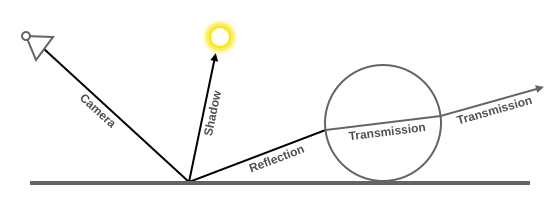
\includegraphics[width=0.7\textwidth]{Images/render_cycles_render-settings_light-paths_rays.png}
\caption{\label{light-path}Light path diagram \href{https://docs.blender.org/manual/en/latest/render/cycles/render\_settings/light\_paths.html}{(Source)}}
\end{figure}
\texttt{Cycles} is a physically based backwards path tracing rendering engine. While
this engine is  physically based, it is not physically correct. It does not aim
to be either \cite{design-goals}.\\

\newpage
\begin{wrapfigure}[19]{r}{0.4\textwidth}
\centering
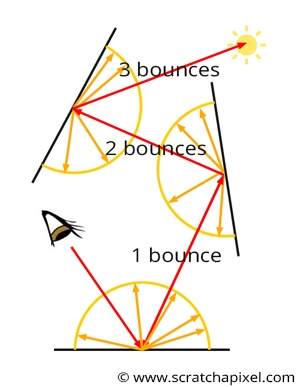
\includegraphics[width=0.35\textwidth]{Images/shad2-globalillum1a.png}
\caption{Backwards path tracer \href{https://www.scratchapixel.com/lessons/3d-basic-rendering/global-illumination-path-tracing}{(Source)}}
\end{wrapfigure}
In backwards path tracers the paths are generated starting from the camera. They
are bounded around the scene until encountering the light source they ``originated'' from.
This is considered an efficient method for direct lighting as a ray will always
yield some result opposed to the forward path tracing where many light rays may
never reach the camera.\\

Cycles offers two integrators, \texttt{Path Tracing} and \texttt{Branched Path Tracing}. Where
\texttt{Branched Path Tracing}  differs is that as a pure path tracer, each bounce of the
light ray bounces in one direction and will pick one light to receive lighting
from, while a \texttt{Branched Path Tracing} will split the path for the first bounce
into multiple rays and sample from multiple lights. Naturally this makes
sampling considerably slower, however it offers lower noise in scenes primarily
lit by a one or single bounce lighting. It is possible to split the ray on
successional bounces as well however the complexity will increase exponentially
for diminishing returns.\\

To combat noise the \texttt{OptiX} denoiser was employed as it operates best on NVIDIA
hardware.\\

Being a jack of all trades Cycles suffers in some areas when compared to
specialised engines such as \texttt{Luxcore}. Specifically Cycles suffers significantly
in advanced light effects such as caustics as explicitly noted in their
documentation \cite{blender-sampling}.\\

\begin{figure}[htbp]
\centering
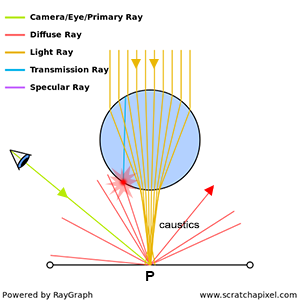
\includegraphics[width=0.4\textwidth]{Images/caustics2.png}
\caption{\label{caustics}Caustics diagram \href{https://www.scratchapixel.com/lessons/3d-basic-rendering/global-illumination-path-tracing}{(Source)}}
\end{figure}
Caustics are the optical phenomenon of light patterns forming on surfaces
through reflections and refraction. These are notably difficult to calculate
efficiently \footnote{There is nothing inherently difficult about caustics, any path tracer can
render them. Instead it is a matter of convergence speed.} using a unidirectional path tracer as many rays will not
collide with the object that should be focusing light. One solution to this is a
technique called photon mapping. In photon mapping an initial pass of the scene
is done using a forwards path tracer to follow the path of light rays as they
interact with glossy and refractive objects.\\

Cycles is significantly slower that \texttt{Eevee} (\texttt{1min vs 16 seconds} for some single
frame renders). With adaptive sampling the number of samples conducted in less
noisy areas is automatically results in a performance improvements.
\paragraph{Thank you to Jack}
\label{sec:orgf00f775}
Due to significant hardware limitations for ray-tracing (\texttt{GTX 760, i5-4670}), a
favour was called in with a good friend, Jack kindly lent his \texttt{RTX 2070}  for a
cycles render. See \href{https://github.com/Jake-Moss/blender-chess/blob/master/Videos/Marble\_cycles.mp4}{master/Videos/Marble\_cycles.mp4}.
\subsubsection{Luxcore}
\label{sec:org58a3ee8}
Another algorithm to calculate caustics is bidirectional path tracing. For each
sample two paths are traced independently using forward and backwards path tracing.
From this every vertex of one path can be connected directly to every vertex of
the other. Weighting all of these sampling strategies using Multiple Importance
Sampling creates a new sampler that can converge faster than unidirectional path
tracing despite the additional work per sample. This works particularly well for
caustics or scenes that are lit primarily through indirect lighting as instead
of connection rays to the camera or source, instead rays are connected to
each other. This allows rays that are very close to form a path \cite{Caustic-Connection}.

\begin{figure}[htbp]
\centering
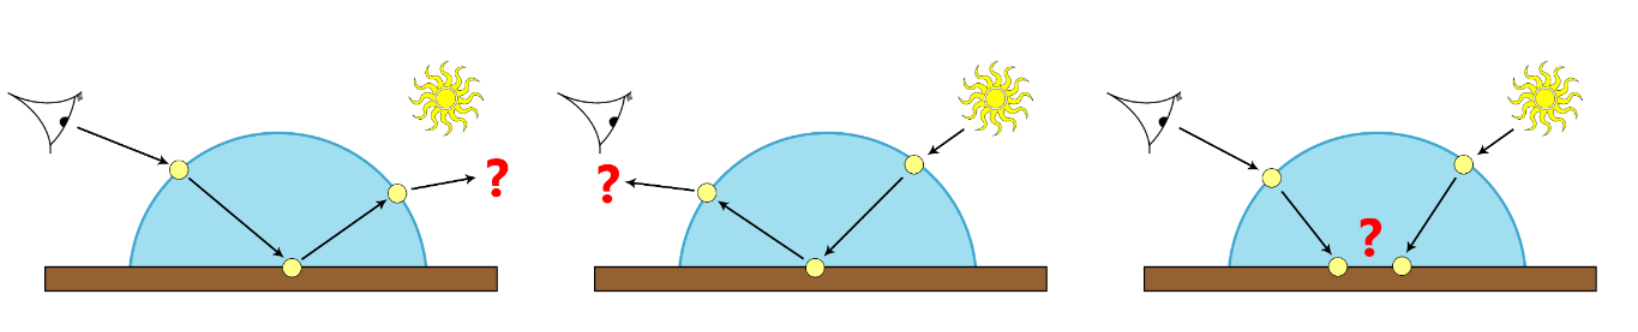
\includegraphics[width=0.7\textwidth]{Images/bidirectional diagram.png}
\caption{\label{bidirectional}Different connection strategies \href{https://graphics.pixar.com/library/CausticConnections/paper.pdf}{(Source)}}
\end{figure}

\texttt{Luxcore} documentation recommends enabling the \texttt{Metropolis sampler} when using
bidirectional path tracing. This allows \texttt{Luxcore} to spend more time sampling
bright areas of the image and thus rendering caustics with greater accuracy.
However, this causes significantly more RAM usage. This was not enabled during
the \texttt{Luxcore} render due to memory restrictions.\\

\texttt{Luxcore} offers caching of caustics through the \texttt{PhotonGI caustic cache} option
however this is only applicable when the scene this static (with the exception of the
camera) and traditional path tracing is used.\\

\texttt{Luxcore} does not finish rendering a scene like \texttt{Eevee} and \texttt{Cycles}, instead
the user must set halt conditions manually. For all renders by within this
report the halt time was set to 10mins. This gave the engine ample time to
converge.
\subsubsection{Tragedy - 22:20, 01/June/2021}
\label{sec:org6038825}
At 10:20pm on the first of June the PC that had been enslaved to rendering a
\texttt{Luxcore} render for more than 96 hours straight, died. Official cause of death is unknown but it
suspected to be something to do with power delivery.\\

A successful data recovery was conducted the next morning. Only the last 12
frames were missing, they were rendered on another device. See
\href{https://github.com/Jake-Moss/blender-chess/blob/master/Videos/disco\_luxcore.mp4}{master/Videos/disco\_luxcore.mp4 }
\section{Python implementation}
\label{sec:org6387c1b}
\subsection{Processing games}
\label{sec:orgb2c64c6}
Reading and stepping through games is handled almost entirely by the chess
library. No special considerations need to be made here. The minium working
example below demonstrates all that is necessary to step through an entire game.

\begin{Code}
\begin{Verbatim}[]
\color[HTML]{383a42}\EFk{import} chess
\EFk{with} \EFb{open}(filename) \EFk{as} \EFv{pgn}:
    game = chess.pgn.read\_game(pgn) \EFcd{\# }\EFct{Parses pgn file}
    \EFv{board} = game.board()

    \EFk{for} move \EFk{in} game.mainline\_moves():
        board.push(move) \EFcd{\# }\EFct{Pushs the move to the move stack, this "makes" the move}
\end{Verbatim}
\end{Code}
\subsection{Pairing problem}
\label{sec:org76aed27}
During a game of chess there is nothing in between moves, simply one discrete
board state after another. This is also how the chess library makes moves, by
computing differences and tracking board states, while this is reliable and
simple it does not play nice when games become continuous (animated).

Initially this script also tracked the board state using a dictionary, with the
square as the key, and corresponding blender object as the value, pushing and
pop at each move. However, this presented difficulties when implementing
animations and special moves. The code was generally cluttered
and not up to an acceptable quality.
\subsection{The solution}
\label{sec:org1e445c8}
To remedy the mentioned problems a custom class was devised, and aptly name
\texttt{CustomPiece}. This class acts as a generalised representation of a piece which
is able to act upon itself and the Blender model it puppets. Stored within an
unrolled 2d array with the index representing its position on the chess board
(See \hyperref[sec:org3045217]{Python implementation - Array Index to world space}) the object is able to
move itself within the array while handling move and capture animations. Special
move handling is generalised into the main loop, (See \hyperref[sec:org274f0d1]{Python implementation -
Special moves}).

This design approach has clear advantages such as
\begin{itemize}
\item Adheres to the \texttt{Model-View-Controller} design philosophy.
\item Array and object manipulation is not handled at any higher level than required.
\item Translation between the chess library interface and Blenders API is seamless.
\item Creates a unique object that pairs a Blender model to a \texttt{python-chess}
\texttt{PieceType}.
\end{itemize}
However, the self-referential nature of objects manipulating the array their
are stored in adds significantly to the complexity. Luckily the implementation is
simple.

An initial sketch of this class can be seen here \ref{class-sketch}.

Implementation can be see here \ref{class-src}.
\subsection{Array index to world space}
\label{sec:org3045217}
\texttt{python-chess} provides great functionality to retrieve what square a move is
coming from, and going to. Internally this is stored as a \texttt{int} representing
each square in 1d array notation.

\begin{minipage}{0.5\textwidth}
\begin{Code}
\begin{Verbatim}[]
\color[HTML]{383a42}\EFv{Square} = \EFb{int}
\EFv{SQUARES} = [
    A1, B1, C1, D1, E1, F1, G1, H1,
    A2, B2, C2, D2, E2, F2, G2, H2,
    A3, B3, C3, D3, E3, F3, G3, H3,
    A4, B4, C4, D4, E4, F4, G4, H4,
    A5, B5, C5, D5, E5, F5, G5, H5,
    A6, B6, C6, D6, E6, F6, G6, H6,
    A7, B7, C7, D7, E7, F7, G7, H7,
    A8, B8, C8, D8, E8, F8, G8, H8,
] = \EFb{range}(\EFhn{64})
\end{Verbatim}
\end{Code}
\end{minipage}
\begin{minipage}{0.5\textwidth}
\setchessboard{color=black,clearboard,showmover=false}
\chessboard[
pgfstyle=
{[base,at={\pgfpoint{0pt}{-0.3ex}}]text},
text= \fontsize{1.2ex}{1.2ex}\bfseries
\sffamily\getfieldnumber\currentwq,
markboard]
\end{minipage}
\newpage
\begin{figure}[htbp]
\centering
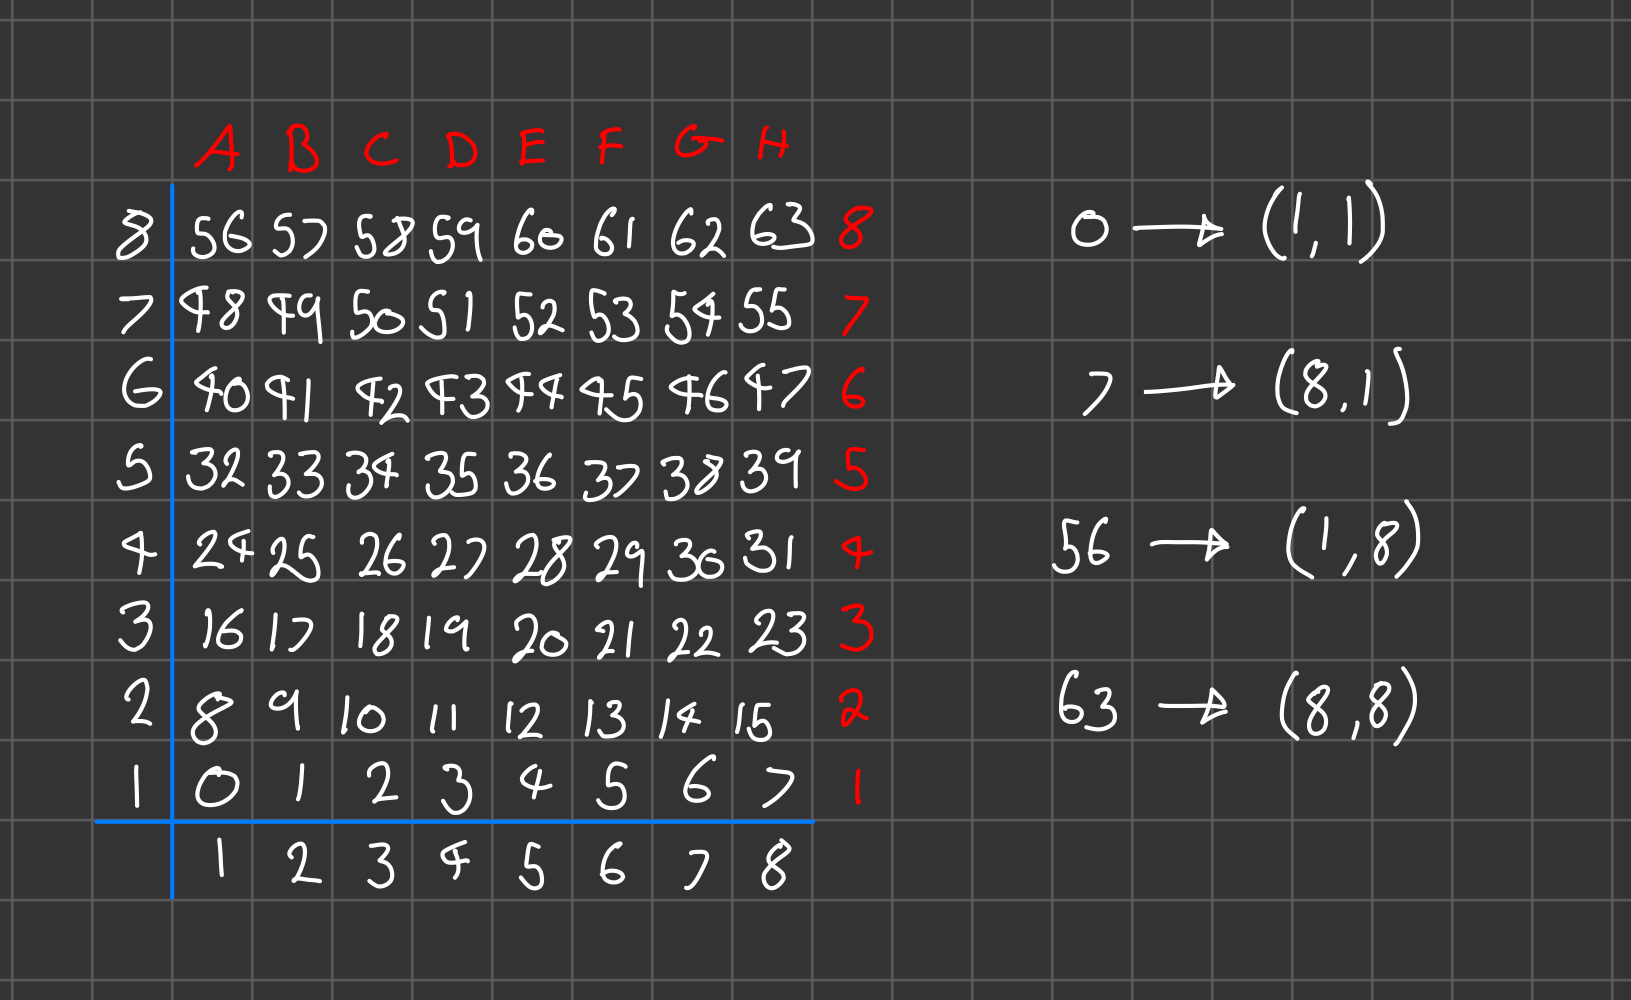
\includegraphics[width=0.5\textwidth]{Images/array.png}
\caption{\label{array-working}Array representation ((\texttt{tl}) Source code, (\texttt{tr}) Chess board, (\texttt{b}) Overlaid)}
\end{figure}

To convert from array indexing two simple expressions were used.
\[x = (\text{INDEX mod } 8) + 0.5\]
\[y = (\text{INDEX div } 8) + 0.5\]\footnote{Note \texttt{div} here is integer division.}
Note the addition of \(0.5\) is to centre the pieces on the board squares in
world space and will be excluded from further examples.
\subsubsection{Abuse of this functionality}
\label{sec:org1fa3750}
\begin{wrapfigure}[14]{r}{0.4\textwidth}
\centering
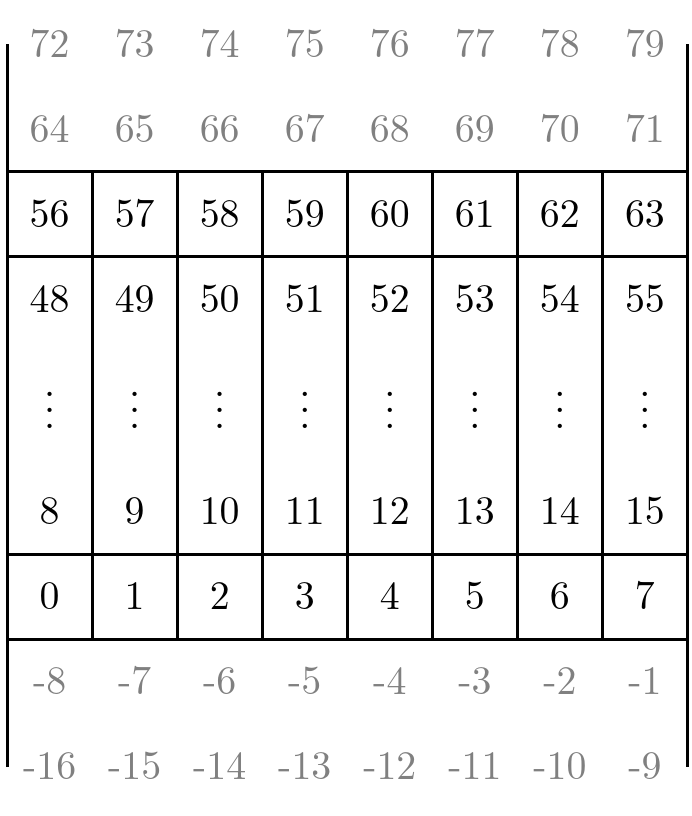
\includegraphics[width=0.35\textwidth]{Images/tikzit_image0.png}
\caption{\label{extended-array}Extended conversion}
\end{wrapfigure}

While modulo will always produce a positive integer between \(0 \to 7\), integer
division can result in negative numbers and is not bounded. Using this the mapping
can be extended past the board it was designed for.

This provides an easy method to place captured pieces after their animation. By
storing each pieces initial position, and adding or subtracting \(16\) depending on
the colour, pieces can be placed \(2\) rows behind their initial position.

Two rows behind was preferable to the respective position on the other side of
the board to avoid the inversion required so that the pawns would be in front of the
back rank pieces.

\newpage
\subsection{Special moves}
\label{sec:org274f0d1}
Figure \ref{flowchart} shows the main loop logic, used to move the correct pieces.
\begin{figure}[htbp]
\centering
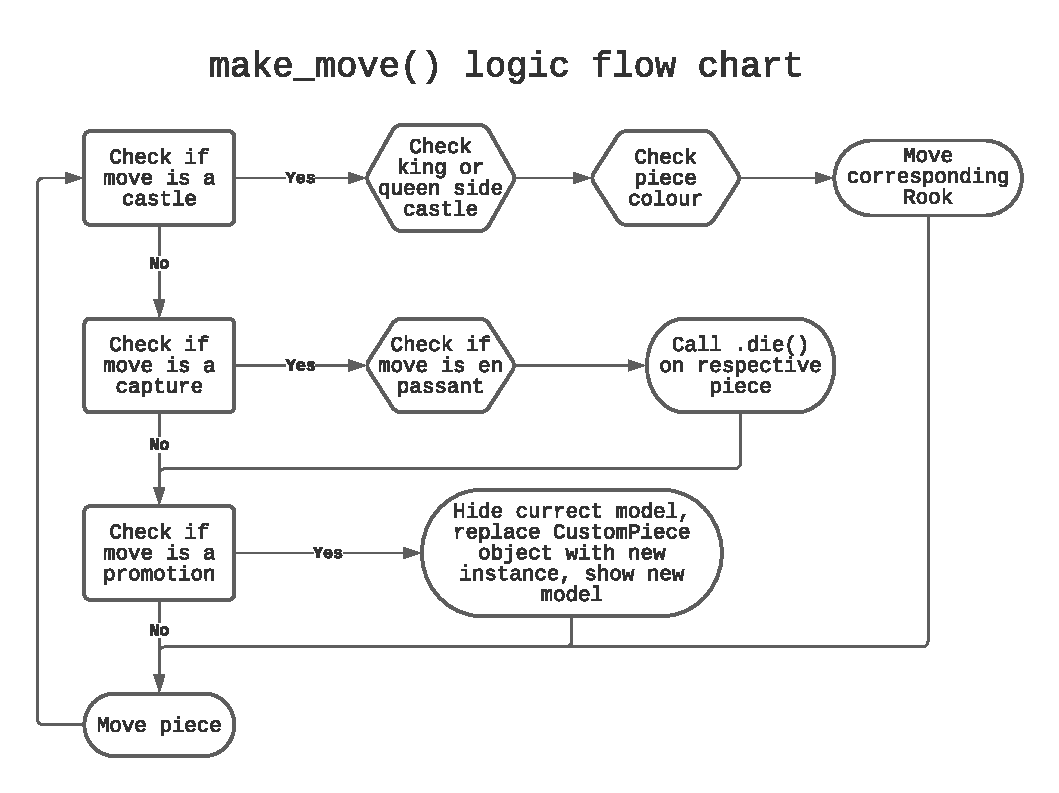
\includegraphics[width=\textwidth]{flowchart.pdf}
\caption{\label{flowchart}Main loop logic}
\end{figure}
\subsubsection{Castling}
\label{sec:orge6d1799}
Within standard chess there are only four castling possibilities, these are easy
enough to check naively. This is the only section that limits this script to
standard chess. To extend support to \texttt{chess960}, a bit-board mask of all the
rooks with castling rights could be filtered to obtain the index of the rook
that will be castled. See \href{https://python-chess.readthedocs.io/en/latest/core.html?highlight=castl\#chess.Board.castling\_rights}{the documentation.}
\begin{Code}
\begin{Verbatim}[]
\color[HTML]{383a42}\EFk{if} board.is\_castling(move):
    \EFk{if} board.turn: \EFcd{\# }\EFct{White}
        \EFk{if} board.is\_kingside\_castling(move):
            array[chess.H1].move(chess.F1)
        \EFk{else}: \EFcd{\# }\EFct{queen side}
            array[chess.A1].move(chess.D1)
    \EFk{else}: \EFcd{\# }\EFct{Black}
        \EFk{if} board.is\_kingside\_castling(move):
            array[chess.H8].move(chess.F8)
        \EFk{else}: \EFcd{\# }\EFct{queen side}
            array[chess.A8].move(chess.D8)
\end{Verbatim}
\end{Code}
\subsubsection{En passant}
\label{sec:org6c3120c}
The \texttt{python-chess} library makes handling en passant a breeze. The move is
checked if it is an en passant first, then as only one square is possible for an
en passant on any move that position is retrieved.
\begin{Code}
\begin{Verbatim}[]
\color[HTML]{383a42}    \EFk{else}: \EFcd{\# }\EFct{standard case}
        \EFk{if} board.is\_capture(move):\EFcd{\# }\EFct{is en passant, great...}
            \EFk{if} board.is\_en\_passant(move):
                array[board.ep\_square].die() \EFcd{\# }\textcolor[HTML]{c3e88d}{\textbf{NOTE}}\EFct{, object is gc'ed}
            \EFk{else}: \EFcd{\# }\EFct{its a normal capture}
                array[locTo].die() \EFcd{\# }\textcolor[HTML]{c3e88d}{\textbf{NOTE}}\EFct{, object is gc'ed}
\end{Verbatim}
\end{Code}
\subsubsection{Promotion}
\label{sec:org157df4f}
Contained within a separate conditional is the promotion logic. This is handled
separately from the rest of the logic as a move can be both a capture and a
promotion.
\begin{Code}
\begin{Verbatim}[]
\color[HTML]{383a42}    array[locFrom].move(locTo) \EFcd{\# }\textcolor[HTML]{c3e88d}{\textbf{NOTE}}\EFct{, piece moves always}

    \EFk{if} move.promotion \EFk{is} \EFk{not} \EFc{None}:
        array[locTo].keyframe\_insert(data\_path=\EFs{"location"}, index=-\EFhn{1})
        array[locTo].hide\_now() \EFcd{\# }\EFct{hide\_now unlinks within blender}
        pieceType = move.promotion \EFcd{\# }\EFct{piece type promoting to}
        array[\EFv{locTo}] = CustomPiece(chess.Piece(pieceType, board.turn),\char92{}
                                   SOURCE\_PIECES[chess.piece\_symbol(pieceType)],\char92{}
                                   array, locTo) \EFcd{\# }\EFct{shiny new object}
        array[locTo].show\_now()
\end{Verbatim}
\end{Code}
A new key-frame is inserted initially as the piece that will promote has already
been moved and the animation needs to finish before it can be hidden.

Within the Blender view port the pieces that will be promoted to already exist
at the right position. This can cause double plaining, however they are not
rendered until needed.
\subsection{Animation}
\label{sec:org10ff813}
\subsubsection{Key frames}
\label{sec:orgc50e98a}
To animate an object within blender two key-frames must be inserted with
different values for some property at varying times. Blender will
interpolate between them (See \hyperref[sec:orge070c77]{Python implementation - Interpolation} for
interpolation methods)

Key-frames for all pieces are inserted every move. This is done to ensure
stationary pieces stay stationary. For every move the piece has \(10\) frames to
complete its moving animation. Between each move there is a \(3\) frame buffer to provide
some separation between moves.

In addition to piece animations, the camera also rotates at a rate of
\(2^{\circ}\) per \(13\) frames.
\begin{Code}
\begin{Verbatim}[]
\color[HTML]{383a42}        \EFv{FRAME\_COUNT} = \EFhn{0}
        keyframes(array) \EFcd{\# }\EFct{intial pos}
        \EFv{FRAME\_COUNT} += \EFhn{10}
        \EFk{for} move \EFk{in} game.mainline\_moves():
            scene.frame\_set(FRAME\_COUNT)

            make\_move(board, move, array)
            keyframes(array) \EFcd{\# }\EFct{update blender}

            camera\_parent.\EFv{rotation\_euler}[\EFhn{2}] += radians(\EFhn{2}) \EFcd{\#}\EFct{XYZ}
            camera\_parent.keyframe\_insert(data\_path=\EFs{"rotation\_euler"}, index=-\EFhn{1})

            board.push(move) \EFcd{\# }\EFct{update python-chess}

            FRAME\_COUNT += \EFhn{10}
            keyframes(array) \EFcd{\# }\EFct{update blender}
            FRAME\_COUNT += \EFhn{3}
\end{Verbatim}
\end{Code}

While the camera's rotation is tied to the length of the game, in order to
continue spinning while the remaining animations (confetti and captures) finish additional key frames
are added. Confetti is conditionally added to the winning king. No confetti for a draw.
\begin{Code}
\begin{Verbatim}[]
\color[HTML]{383a42}        \EFv{confetti} = bpy.data.collections[\EFs{"Board"}].objects[\EFs{'Confetti source'}]
        \EFk{if} board.outcome() \EFk{is} \EFk{not} \EFc{None}:
            winner = board.outcome().winner
            \EFv{king\_square} = board.king(winner)
            \EFv{xTo}, \EFv{yTo} = square\_to\_world\_space(king\_square)
            confetti.\EFv{location} = Vector((xTo, yTo, \EFhn{3}))
            bpy.data.particles[\EFs{"Confetti"}].\EFv{frame\_start} = FRAME\_COUNT
            bpy.data.particles[\EFs{"Confetti"}].\EFv{frame\_end} = FRAME\_COUNT + \EFhn{12}

        \EFk{print}(FRAME\_COUNT)
        \EFk{for} \_ \EFk{in} \EFb{range}(\EFhn{5}):
            scene.frame\_set(FRAME\_COUNT)
            camera\_parent.\EFv{rotation\_euler}[\EFhn{2}] += radians(\EFhn{2}) \EFcd{\#}\EFct{XYZ}
            camera\_parent.keyframe\_insert(data\_path=\EFs{"rotation\_euler"}, index=-\EFhn{1})

            FRAME\_COUNT += \EFhn{13}
\end{Verbatim}
\end{Code}
In order to move the camera with a fixed rotation and radius from the centre of
the board the camera was made a child of a \texttt{Empty Plain Axis}. Rotations and
translations applied to the camera parent are also applied to the camera. This
allows for ease fixed distance rotations.
\begin{figure}[htbp]
\centering
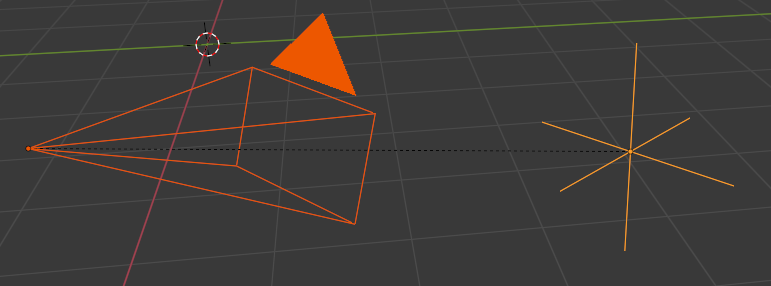
\includegraphics[width=0.5\textwidth]{Images/camera parent.png}
\caption{\label{camera-parent}Camera parent axis}
\end{figure}
\subsubsection{Interpolation}
\label{sec:orge070c77}
Blender offers 3 curves for interpolation between key-frames.
\begin{itemize}
\item Constant\\
Object value only objects on the last possible frame.
\item Linear\\
Object value changes linearly between the key-frames to form piecewise
continuous curve.
\item Bézier\\
The object value is interpolated using a Bézier curve. Bézier curves are
parametric curves used in computer graphics to create smooth surfaces, or in
this case, a smooth function between two points.

Blender implements a forward differencing method for a cubic Bézier curve
evident from the source code \cite{blender-source}.
\end{itemize}
By default Blender uses Bézier curve interpolation for all motions. This is the
preferred option for piece movement. However, linear was opted for as the camera
motion although a cubic Bézier curve would produce the same outcome it made
debugging slightly easier.
\subsection{Reproducibility}
\label{sec:org244aad8}
This project was created used
\begin{itemize}
\item Blender \texttt{2.92}
\url{https://www.blender.org/}
\item Python \texttt{3.9.5} \footnote{Blender comes bundled with this version. If the system python is used
instead ensure it matches the version Blender was built with and is above \texttt{3.7}
for the \texttt{\_\_future\_\_} module. Past \texttt{3.10} the \texttt{\_\_future\_\_} module is no longer required.}
\url{https://www.python.org/}
\item python-chess \texttt{1.5.0} \footnote{This project requires the \texttt{Outcome} class released in \texttt{1.5.0}}
\url{https://github.com/niklasf/python-chess}
\end{itemize}
\subsubsection{Python environment}
\label{sec:org4ac9b25}
Blender is distributed with its own python installation for consistency, however
this means that installed python modules are not present
\cite{blender-python-env}. To mitigate this the \texttt{-{}-target} flag for \texttt{pip install}
can be used to install directly to the blender python environment
\cite{pip-install-man}.
\begin{Code}
\begin{Verbatim}[]
\color[HTML]{383a42}pip install -t \char126{}/.config/blender/2.92/scripts/modules chess
\end{Verbatim}
\end{Code}
This ensures Blenders \texttt{Python} will has access to the required libraries for this
script to function.

\section{Results}
\label{sec:org6ce5094}
Animations referenced in this section are available on the \href{https://github.com/Jake-Moss/blender-chess/tree/master/Videos}{public GitHub repo.}
They will be refered to by their filenames\footnote{\texttt{higher/lower} within files names refers to the bit-rate of the assembled images.} and hyperlinked. The still
renders below may not appear within the animations as they may not be suitable
to comparison, instead still renders from the same scenes are included to
showcase these effects. The animations themselves and the appearance of these
effects will be shown within the presentation.

\begin{itemize}
\item \href{https://github.com/Jake-Moss/blender-chess/blob/master/Videos/Marble\_eevee\_higher.mp4}{\texttt{Marble\_eevee.mp4}}\\
This is the complete product. Rendered using \texttt{Eevee}
\item \href{https://github.com/Jake-Moss/blender-chess/blob/master/Videos/Marble\_cycles\_higher.mp4}{\texttt{Marble\_cycles.mp4}}\\
This is the path traced render of the final scene for comparison purposes. The
scene and setup is identical other than the engine.
\item \href{https://github.com/Jake-Moss/blender-chess/blob/master/Videos/Marble\_stacked\_higher.mp4}{Marble\textsubscript{stacked}\textsubscript{higher.mp4}}\\
A side by side comparison between \texttt{Eevee} and \texttt{Cycles}
\item \href{https://github.com/Jake-Moss/blender-chess/blob/master/Videos/disco\_luxcore.mp4}{\texttt{disco\_luxcore.mp4}}\\
Disco chess was set to render long before this project was near completion.
Although it is missing many key aspects and features its purpose is to
demonstrate what bidirectional path tracing can do for caustics. \texttt{Luxcore} has
a few notable incompatibilities with some aspects of the scene. This will be
discussed in the presentation.
\end{itemize}

\begin{figure}[htbp]
\centering
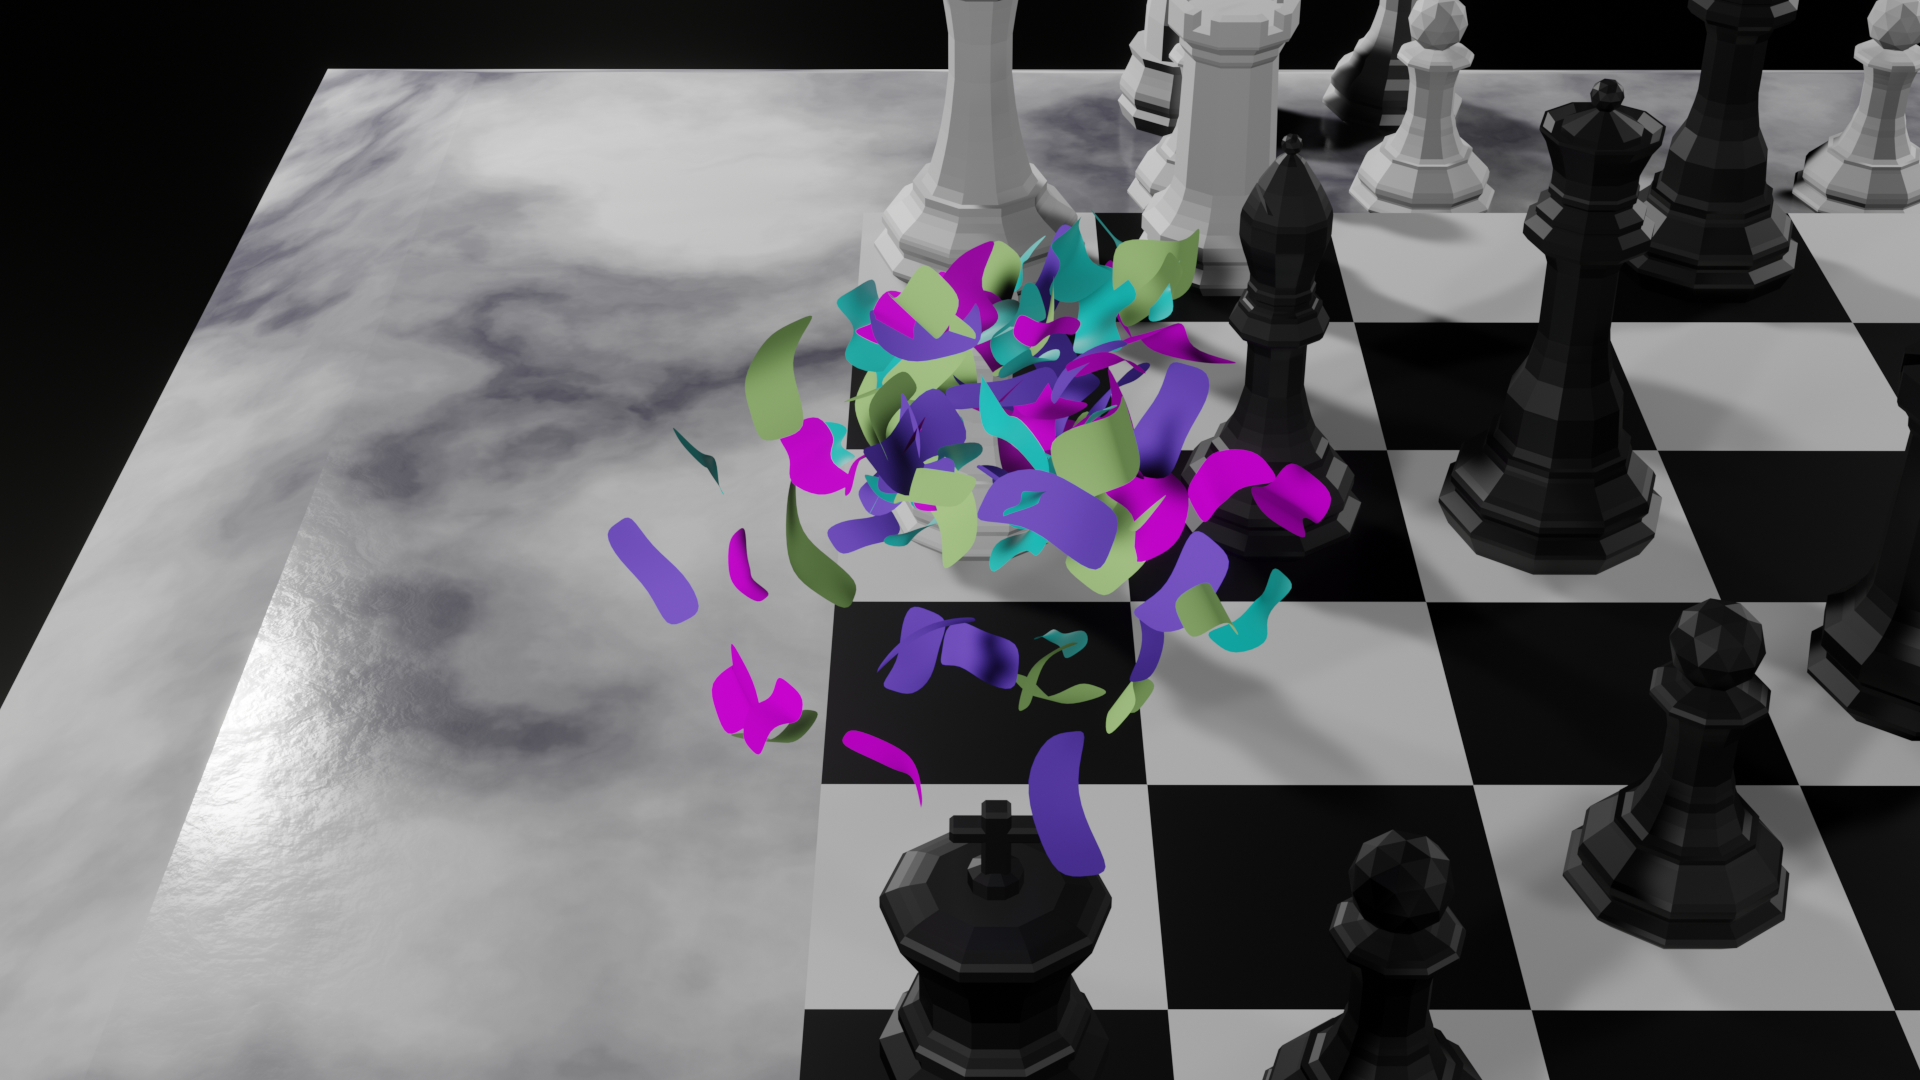
\includegraphics[width=\textwidth]{Images/confetti-eevee.png}
\caption{\label{confetti-eevee}Confetti comparison Eevee}
\end{figure}

\begin{figure}[htbp]
\centering
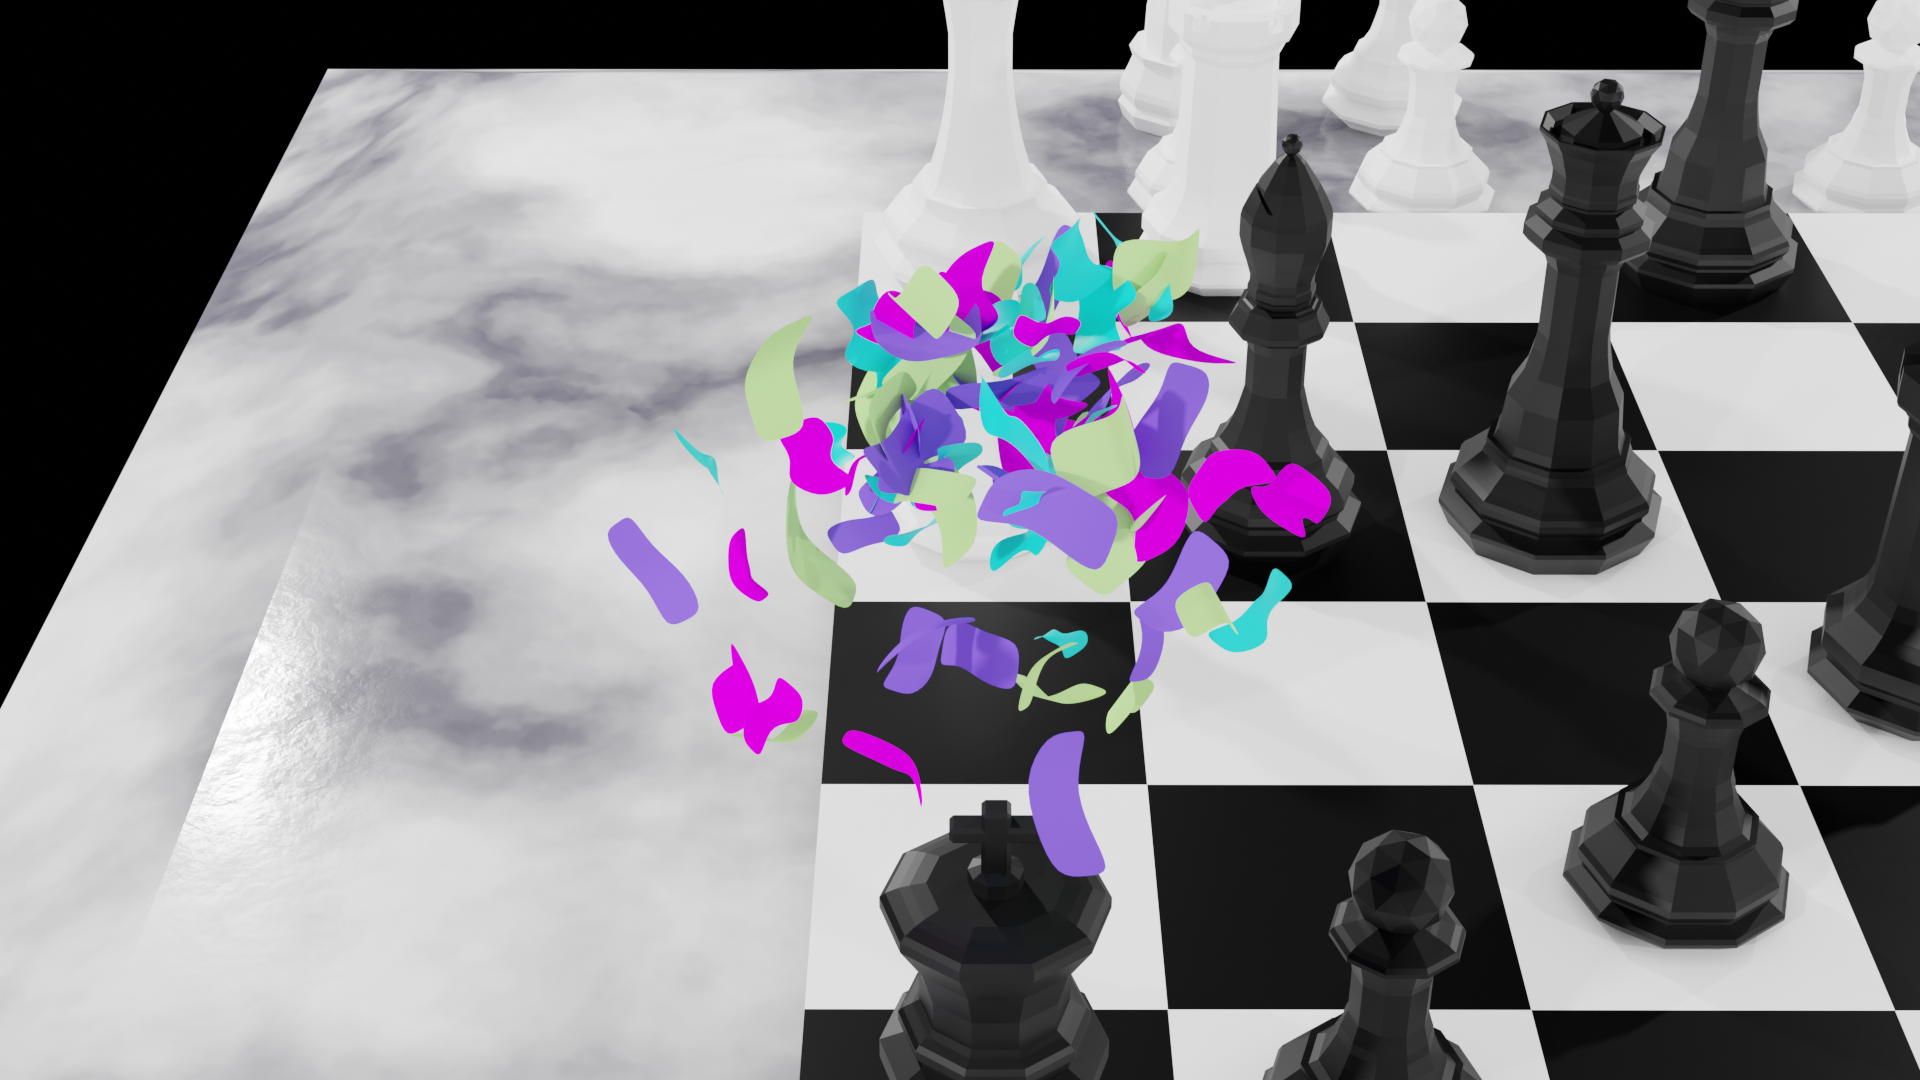
\includegraphics[width=\textwidth]{Images/confetti-cycles.png}
\caption{\label{confetti-cycles}Confetti comparison Cycles}
\end{figure}

\begin{figure}[htbp]
\begin{center}

\includegraphics[width=0.3\textwidth]{Images/confetti-eevee-1.png}

\includegraphics[width=0.3\textwidth]{Images/confetti-eevee-2.png}

\includegraphics[width=0.3\textwidth]{Images/confetti-eevee-3.png}
\end{center}
\caption{\label{confetti-eevee-close}Eevee confetti close up}
\end{figure}
\begin{figure}[htbp]
\begin{center}

\includegraphics[width=0.3\textwidth]{Images/confetti-cycles-1.png}

\includegraphics[width=0.3\textwidth]{Images/confetti-cycles-2.png}

\includegraphics[width=0.3\textwidth]{Images/confetti-cycles-3.png}
\end{center}
\caption{\label{confetti-cycles-close}Cycles confetti close up}
\end{figure}
\newpage
It is clear from the close up figures that \texttt{Cycles} produces significantly more
believable lighting due to its ability to accurately computer indirect lighting.
\texttt{Eevee} tries its best with its approximations of shadows however it fails to
correctly illuminate the arch formed by two other pieces of confetti.\\

Between the two intersection pieces on the right image, \texttt{Cycles} correctly
provides the indirect and ambient occlusion that should be present within such a
formation. \texttt{Eevee} illuminates the whole purple face as if the pink piece was
not present at all. The shadows cast by the pieces are also not present at
all.\\

\texttt{Eevee} also struggles to deal with the twist in the teal piece (left
image), \texttt{Cycles} correctly produces the indirect lighting and shadowing.
\begin{figure}[htbp]
\centering
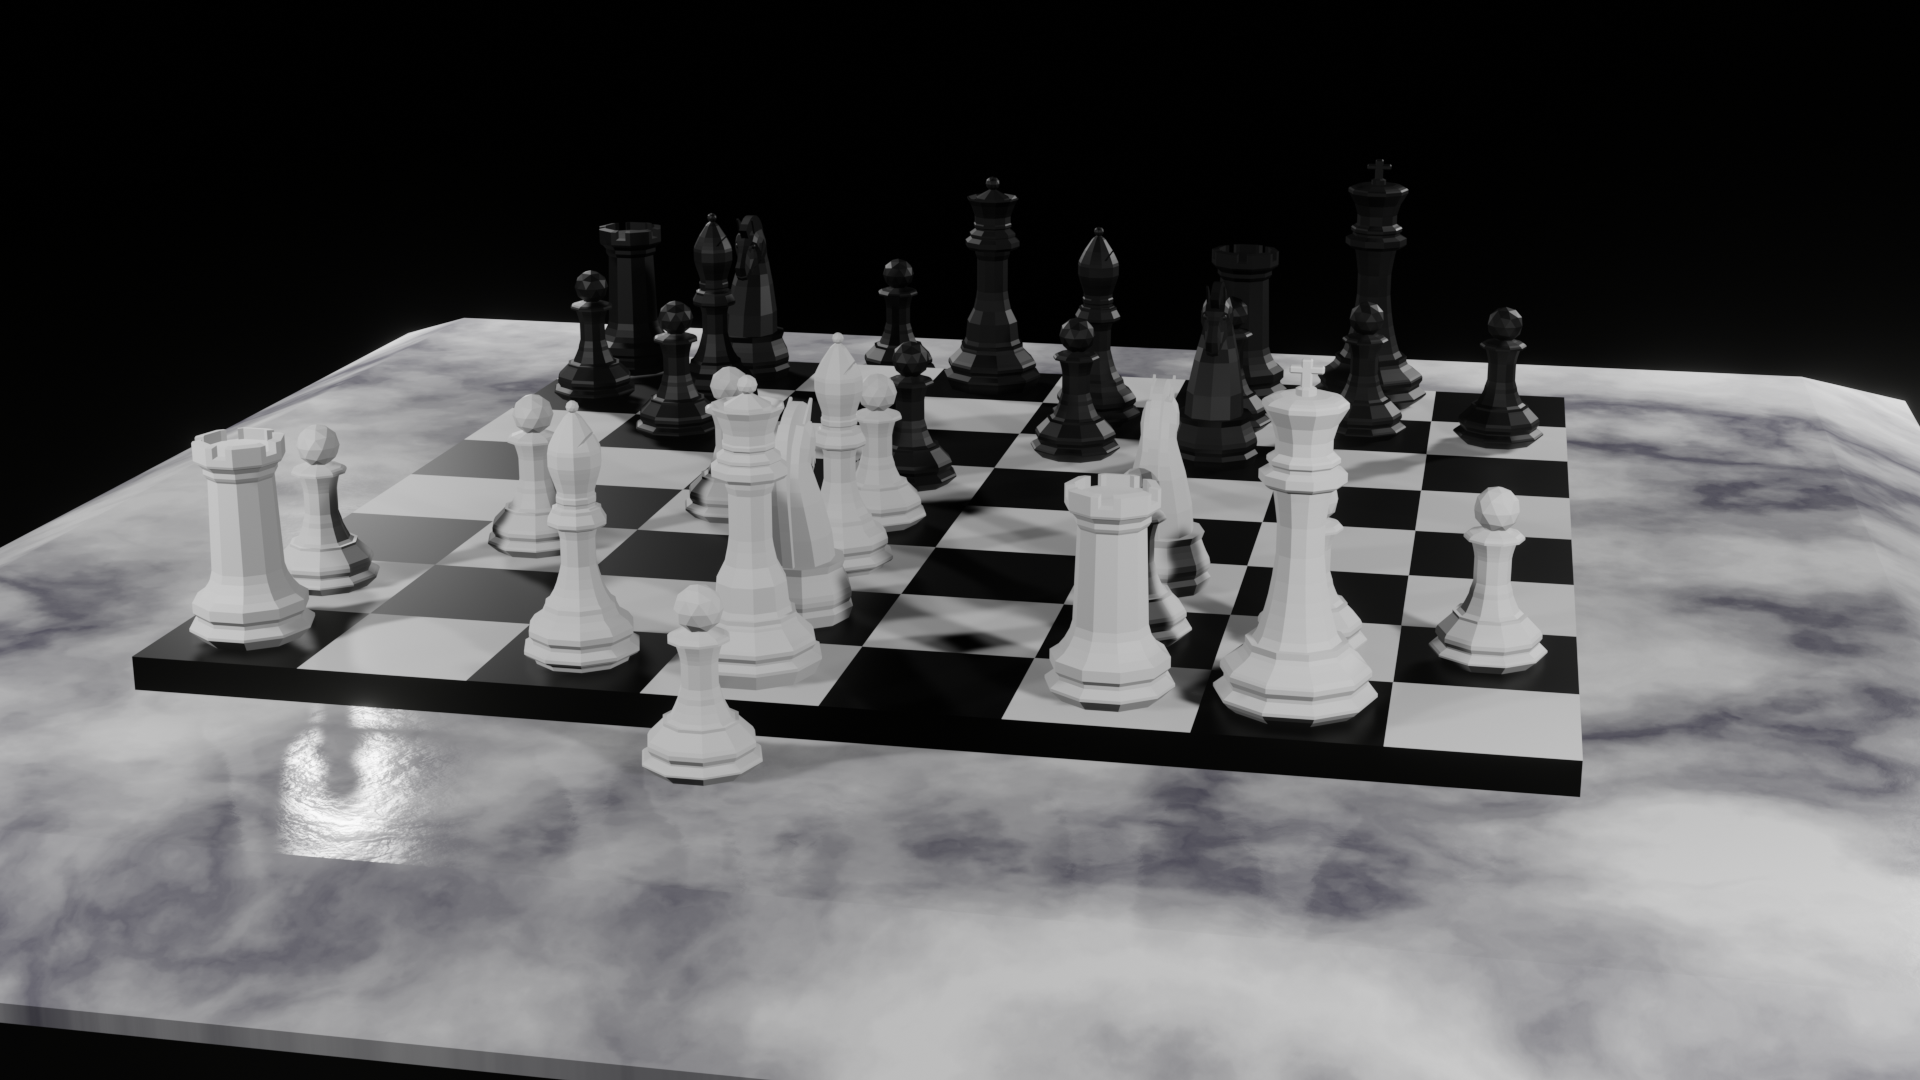
\includegraphics[width=\textwidth]{Images/reflections-eevee.png}
\caption{\label{reflections-eevee}Comparison Eevee}
\end{figure}

\begin{figure}[htbp]
\centering
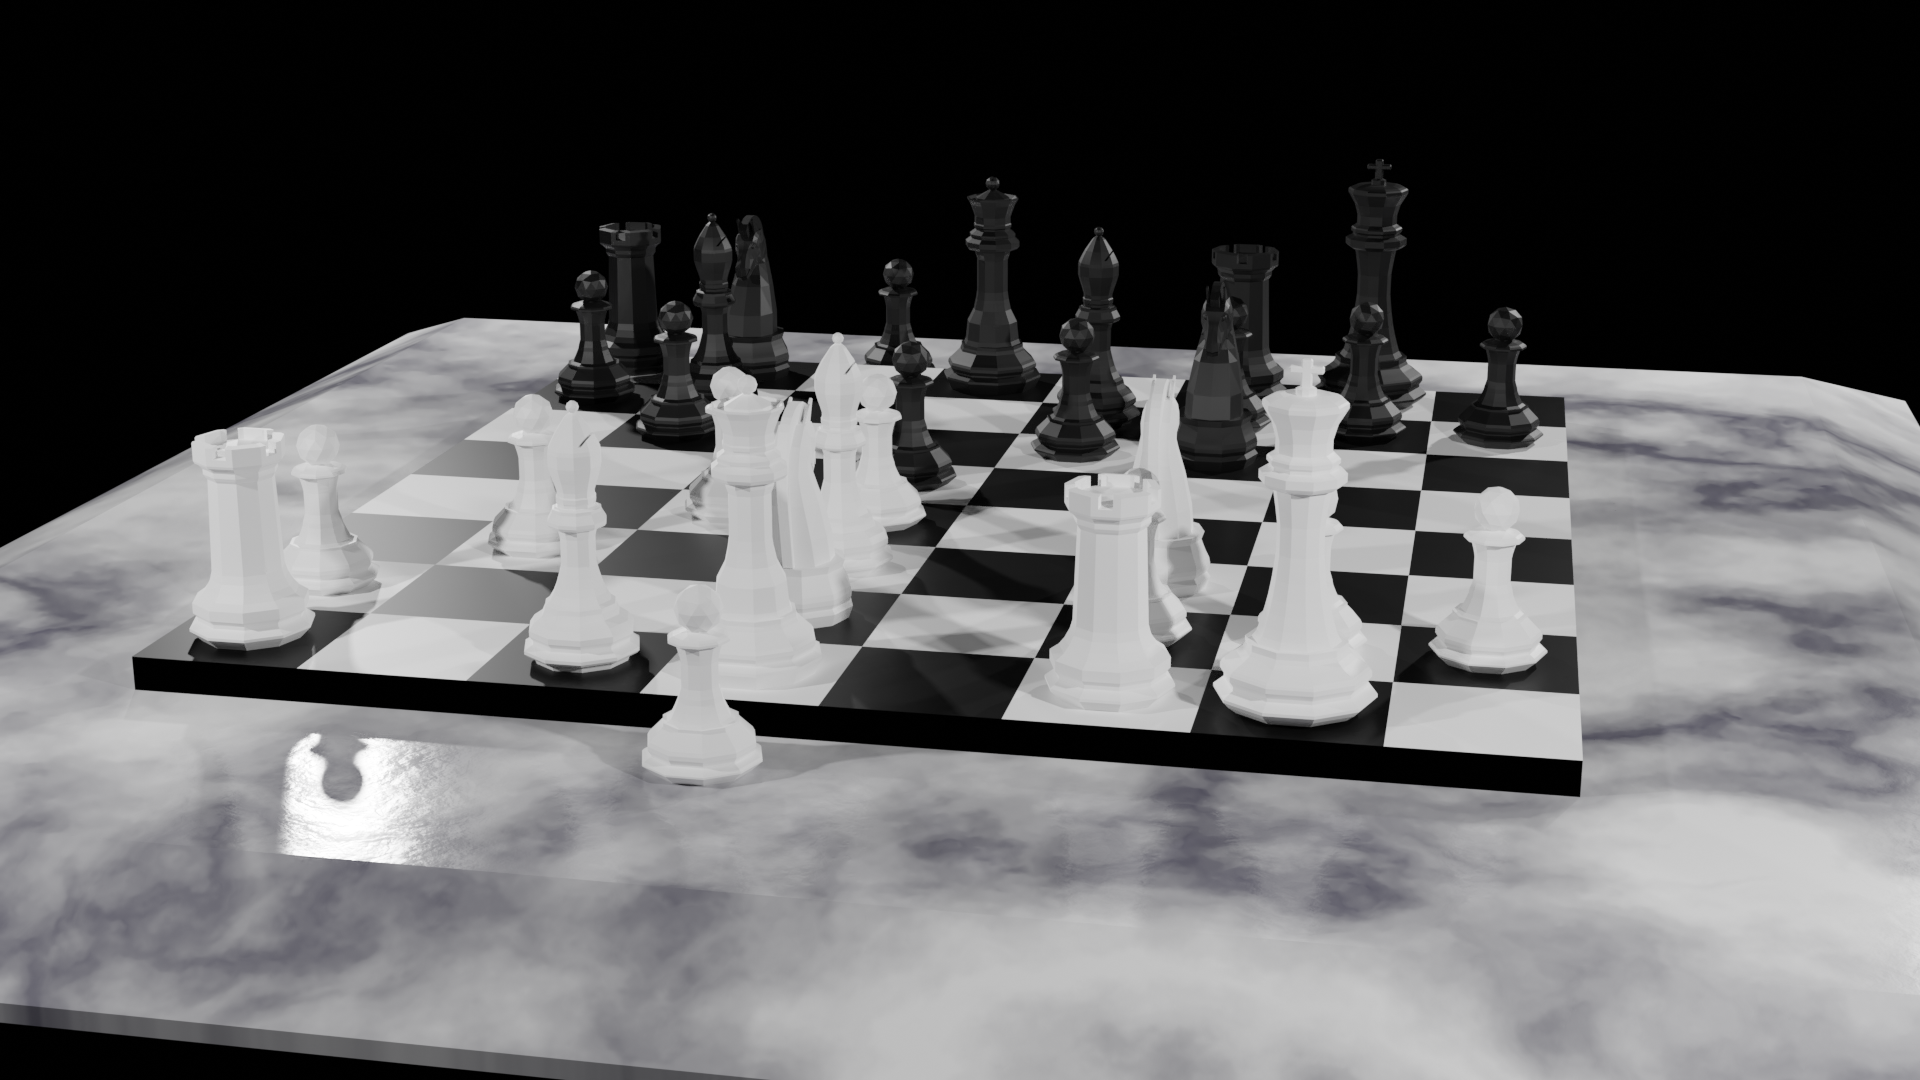
\includegraphics[width=\textwidth]{Images/reflections-cycles.png}
\caption{\label{reflections-cycles}Comparison Cycles}
\end{figure}

\begin{figure}[htbp]
\begin{center}
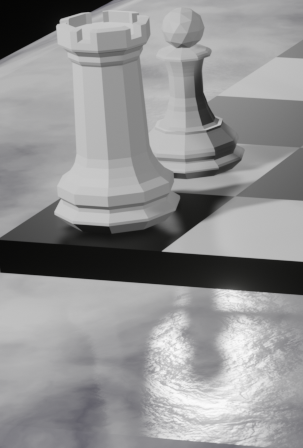
\includegraphics[width=0.3\textwidth]{Images/reflections-eevee-1.png}
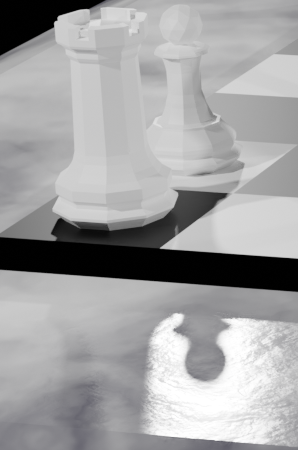
\includegraphics[width=0.3\textwidth]{Images/reflections-cycles-1.png}
\end{center}
\caption{\label{reflections-close}Eevee-Cycles reflections close up}
\end{figure}
\begin{figure}[htbp]
\begin{center}

\includegraphics[width=0.4\textwidth]{Images/reflections-eevee-2.png}

\includegraphics[width=0.4\textwidth]{Images/reflections-cycles-2.png}
\end{center}
\caption{\label{shading-close}Eevee-Cycles shading close up}
\end{figure}
\newpage
In Figure \ref{reflections-close} \texttt{Cycles}'s shadowing and reflectance create a
sharper outline around the pawn. \texttt{Eevee} does not show this as the reflectance
is an approximation using the depth buffer and the previous frame colour.\\

On the space tile \texttt{Cycles} is able to correctly compute the reflection of the
piece in a sharp manner by a material with a mirror like finish.
\texttt{Eevee}'s approximations once again cause the reflections to be blurred.\\

Within the same figure the normal map of the marble texture causes the light to
waver reflect in a non-uniform manner.\\

In Figure \ref{shading-close} \texttt{Eevee} adds shadows without considering indirect
lighting. \texttt{Cycles} produces a more realistic result. The intersection of all the
shadows should not be the sum of its elements as the indirect lighting will
illuminate it partially.

\begin{figure}[htbp]
\centering
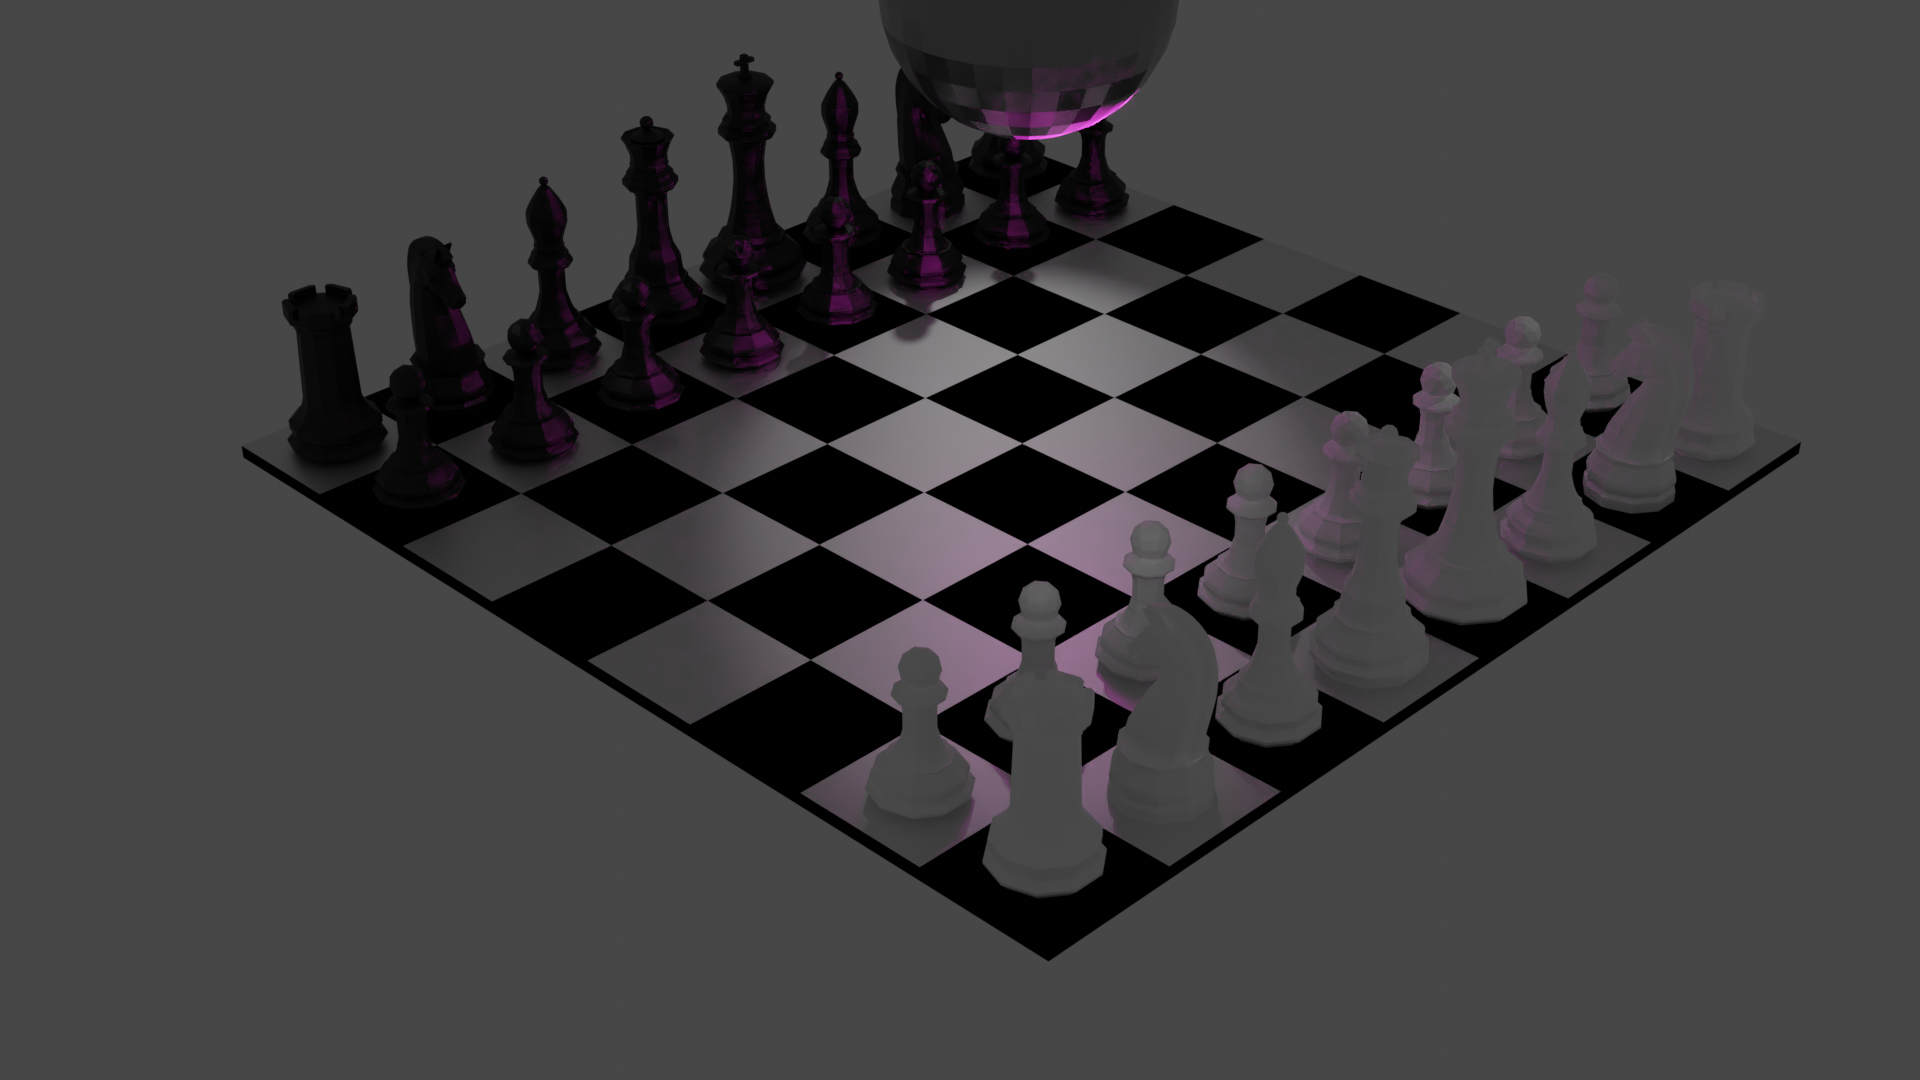
\includegraphics[width=\textwidth]{Images/Disco kinda working.png}
\caption{Cycles attempting disco chess}
\end{figure}

\begin{figure}[htbp]
\centering
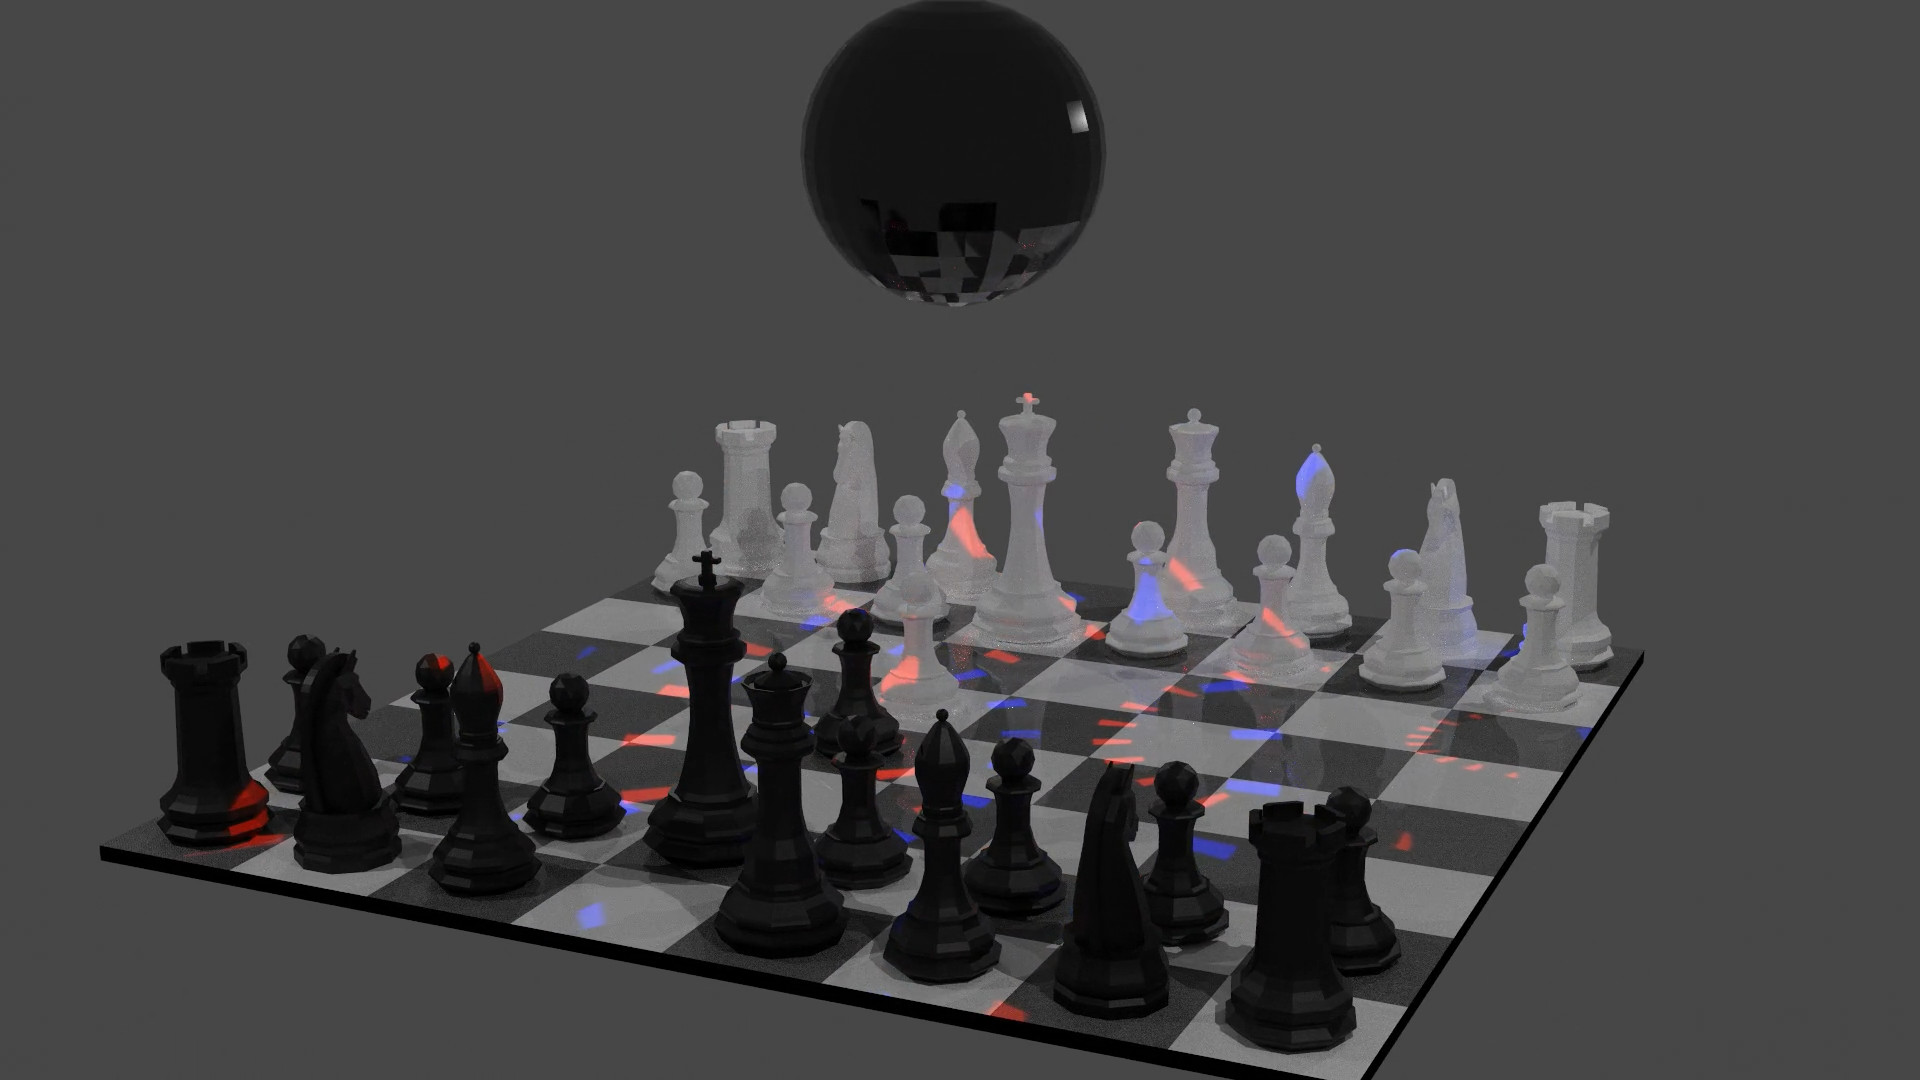
\includegraphics[width=\textwidth]{Images/mpv-shot0001.jpg}
\caption{Luxcore succeeding at disco chess (Frame from \href{https://github.com/Jake-Moss/blender-chess/blob/master/Videos/disco\_luxcore.mp4}{disco\textsubscript{luxcore.mp4}})}
\end{figure}

Some of \texttt{Cycles} backwards rays do make it to the light source, unfortunately
this is not accurate enough for the denoiser not to be fooled, it tries its best
to clean up this noise and creates a faint pink glow on the board an pieces.\\

Due to \texttt{Luxcore}'s bidirectional path tracing it does not suffer from this and
is able to compute the caustics accurately and within a reasonable convergence
time. However, the image is still exceptionally noisy and requires longer
rendering time to reach the noise thresholds of \texttt{Cycles}.

Animations were rendered to individual frames as PNGs, they were then assembled
using \texttt{ffmpeg}.
\begin{Code}
\begin{Verbatim}[]
\color[HTML]{383a42}ffmpeg -framerate \EFhn{24} -s 1920x1080 -i \%04d.png -vcodec libx264 -crf \EFhn{25} -pix\_fmt yuv420p ../Videos/\$\EFv{FILENAME}.mp4
\end{Verbatim}
\end{Code}
\section{Self-evaluation}
\label{sec:orgeb936ed}
\subsection{Avoiding basic errors}
\label{sec:org2686d70}
I believe I have achieved all basic marking criteria and are deserving of all
basic marks. (7 Marks)
\subsection{Further additional marks}
\label{sec:orgd39f525}
In addition to the basic marks I believe I have earned the following marks.
\begin{enumerate}
\item \texttt{Report is well-written and concise}\\
I believe this report is well-written and concise where possible while still covering many
important topics. (1 Mark)
\item \texttt{Report text and image examples support each other well}\\
Images and diagrams were used in conjunction with text to better portray my
ideas and understanding. Screenshots of texture configurations and the
accompanying reasons are an example of this. (1 Mark)
\item \texttt{An ample number of illustrative images are used to clearly demonstrate the
   techniques}\\
I have consistently used images to illustrate concepts and techniques used
along with the results of texture generation, modelling, and rendering. (1 Mark)
\item \texttt{It is evident from the report whether or not the techniques implemented
   were appropriate for achieving the task}\\
I believe I used appropriate techniques to create a visually appealing
model. For example, \texttt{MIS, Screen Space Reflections, Adaptive Sample,
   and Caustics} are relevant to the project and work to create a visually
appealing animation. (1 Mark)
\item \texttt{Techniques chosen were carefully considered and compared with alternatives
   demonstrating insight into the design decision process}\\
I chose techniques thought to best demonstrate adequate knowledge while
working towards a visually appealing  result. Many features and algorithms
were consider which are more physically correct or such but were not considered cost
worthy or feasible. (1 Mark)
\item \texttt{Report demonstrates significant work testing and applying techniques}\\
Throughout this report I have shown significant testing through the
application and comparison of techniques including differences between
rendering engines and their effect on caustics. (1 Mark)
\item \texttt{The report demonstrates that independent research extending beyond the specific course taught techniques have contributed to the final project in a meaningful way}\\
I have delved into the source of Blender to find methods and algorithms used
where I found documentation to be lacking. I found, read, and cited original
papers detailing \texttt{GGX, MSGGX, Christensen-Burley model, and Random walk
   model}. (2 Marks)
\item \texttt{Large variety of techniques applied}\\
I have used;
\begin{itemize}
\item Procedural texture and normal map generation using noise functions
\item Particle systems and explosion
\item Direct and indirect lighting
\item Reflections, bloom, specular reflection and other lighting effects
\item Advanced lighting techniques (caustics)
\item A variety of rendering algorithms including rasterization, path tracing,
and bidirectional path tracing
\end{itemize}
(2 Marks)
\item \texttt{Final product looks visually appealing and complete}\\
Throughout this project I always aimed to create something visually appealing.
I believe I have excelled at this and made something I would display
publicly with pride. (2 Marks)
\end{enumerate}

\newpage
\section{Appendix}
\label{sec:org357c765}
\begin{figure}[htbp]
\centering
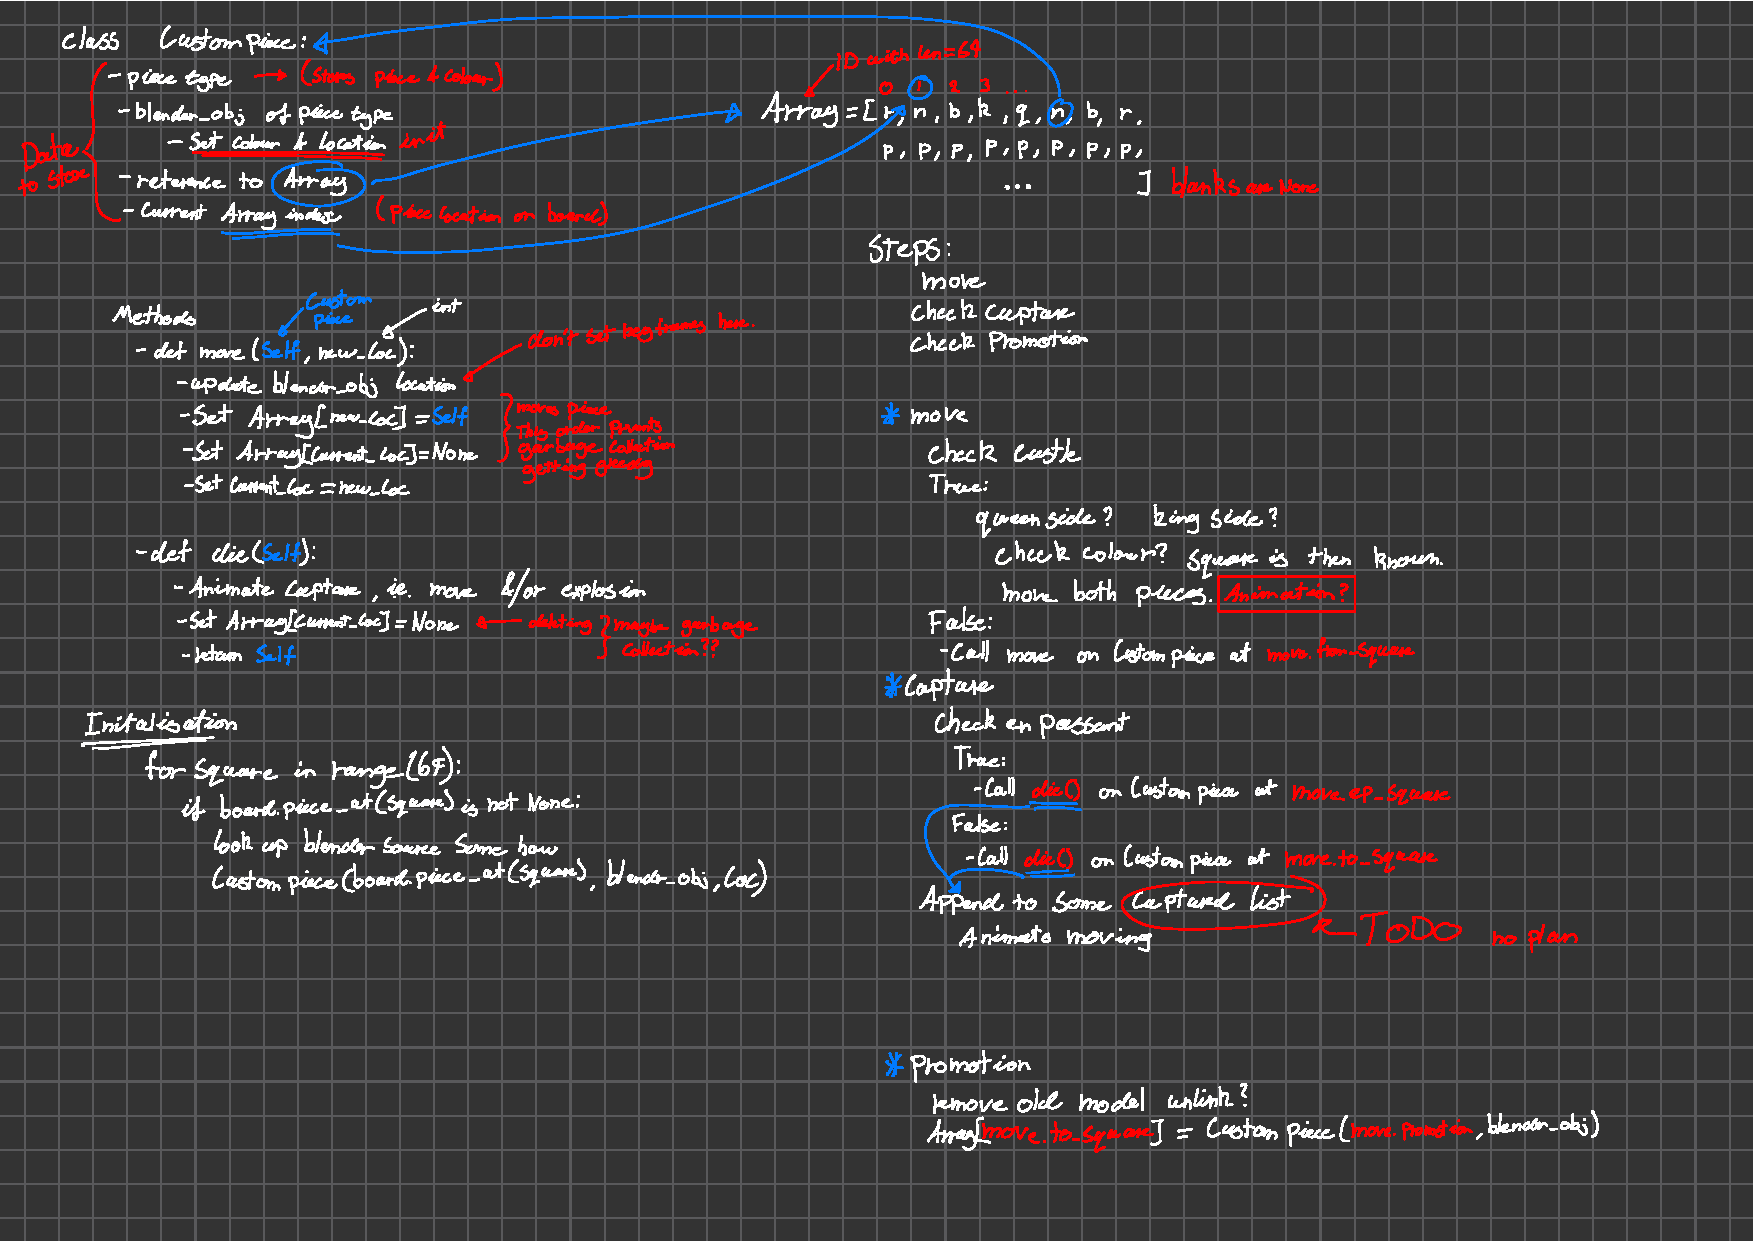
\includegraphics[width=\textwidth]{Scratchpad.pdf}
\caption{\label{class-sketch}\texttt{CustomPiece} Initial sketch}
\end{figure}

\begin{Code}
\begin{Verbatim}[]
\color[HTML]{383a42}\EFk{class} \EFt{CustomPiece}():
    \EFk{def} \EFf{\_\_init\_\_}(\EFk{self}, \EFv{pieceType}: chess.Piece, blender\_obj: bpy.types.Object,\char92{}
                 array: List[Optional[CustomPiece]], loc: \EFb{int}):
        \EFk{self}.\_pieceType = pieceType.piece\_type \EFcd{\# }\EFct{int}
        \EFk{self}.\EFv{\_colour} = pieceType.color         \EFcd{\# }\EFct{bool}
        \EFk{self}.\EFv{\_blender\_obj} = blender\_obj.copy()
        \EFk{self}.\EFv{\_array} = array                    \EFcd{\# }\EFct{reference to array containing self}
        \EFk{self}.\EFv{\_inital\_loc} = loc
        \EFk{self}.\EFv{\_loc} = loc                        \EFcd{\# }\EFct{int (1d array index)}

        \EFv{x}, \EFv{y} = square\_to\_world\_space(\EFk{self}.\_loc)
        \EFk{self}.\_blender\_obj.\EFv{location} = Vector((x, y, \EFhn{0.3}))

        \EFcd{\# }\EFct{set material based on colour}
        \EFk{if} \EFk{self}.\EFv{\_colour}:
            \EFk{self}.\_mat = bpy.data.materials[\EFs{"White pieces"}]
        \EFk{else}:
            \EFk{self}.\_mat = bpy.data.materials[\EFs{"Black pieces"}]
        \EFk{self}.\_blender\_obj.\EFv{active\_material} = \EFk{self}.\_mat


        \EFk{if} \EFk{self}.\_colour \EFk{and} \EFk{self}.\_pieceType == chess.KNIGHT:
            \EFk{self}.\_blender\_obj.rotation\_euler[\EFhn{2}] = radians(\EFhn{180}) \EFcd{\#}\EFct{XYZ}
        \EFcd{\# }\EFct{add object to collection so its visable}
        bpy.data.collections[[\EFs{'Black'}, \EFs{'White'}][\EFk{self}.\_colour]].objects.link(\EFk{self}.\_blender\_obj)

    \EFk{def} \EFf{move}(\EFk{self}, new\_loc: \EFb{int}, zTo: \EFb{float} = \EFhn{0.3}):
        \EFv{xTo}, \EFv{yTo} = square\_to\_world\_space(new\_loc)
        \EFk{self}.\_blender\_obj.location = Vector((xTo, yTo, zTo))
        \EFk{print}(\EFs{"Moved to "}, \EFk{self}.\_blender\_obj.location)

        \EFk{self}.\_array[\EFv{new\_loc}] = \EFk{self}
        \EFk{self}.\_array[\EFk{self}.\EFv{\_loc}] = \EFc{None}

        \EFk{self}.\_loc = new\_loc

    \EFk{def} \EFf{die}(\EFk{self}) -> CustomPiece:
        \EFk{self}.\_array[\EFk{self}.\EFv{\_loc}] = \EFc{None}
        \EFk{self}.keyframe\_insert(data\_path=\EFs{"location"}, frame=FRAME\_COUNT-\EFhn{6})

        \EFv{xTo}, \EFv{yTo} = square\_to\_world\_space(\EFk{self}.\_loc)
        \EFk{self}.\_blender\_obj.location = Vector((xTo, yTo, \EFhn{2.1}))
        \EFk{self}.keyframe\_insert(data\_path=\EFs{"location"}, frame=FRAME\_COUNT+\EFhn{3})

        \EFk{if} \EFk{self}.\_colour:
            \EFk{self}.\_inital\_loc += -\EFhn{16}
        \EFk{else}:
            \EFk{self}.\_inital\_loc += \EFhn{16}

        \EFv{xTo}, \EFv{yTo} = square\_to\_world\_space(\EFk{self}.\_inital\_loc)
        \EFk{self}.\_blender\_obj.location = Vector((xTo, yTo, \EFhn{2.1}))
        \EFk{self}.keyframe\_insert(data\_path=\EFs{"location"}, frame=FRAME\_COUNT+\EFhn{21})

        \EFv{xTo}, \EFv{yTo} = square\_to\_world\_space(\EFk{self}.\_inital\_loc)
        \EFk{self}.\_blender\_obj.location = Vector((xTo, yTo, \EFhn{0.1}))
        \EFk{self}.keyframe\_insert(data\_path=\EFs{"location"}, frame=FRAME\_COUNT+\EFhn{29})

        \EFk{return} \EFk{self}
\end{Verbatim}
\end{Code}
\label{class-src}

\newpage
\printbibliography
\end{document}
